\documentclass{book}

\usepackage[x11names]{xcolor}
\usepackage{pdfpages}
\usepackage{hyperref}
\usepackage[utf8]{inputenc}
\usepackage[czech]{babel}
\usepackage[T1]{fontenc}
\usepackage{amsmath}
\usepackage{amsfonts}
\usepackage{amssymb}
\usepackage{delarray}
\usepackage{float}
\usepackage[left=2cm,right=2cm,top=2cm,bottom=2cm]{geometry}				

% code samples
\usepackage{listings}
\usepackage{courier}
%\lstset{basicstyle=\footnotesize\ttfamily,breaklines=true}
\lstset{
    basicstyle=\ttfamily\footnotesize,
    breaklines=true,
    frame=single, % adds a frame around the code
    xleftmargin=2cm,
    xrightmargin=2cm,
}

% exercises and solutions
\usepackage{mdframed}
\newmdenv[topline=false, bottomline=false, skipabove=\topsep, rightline=false,
  skipbelow=\topsep]{exercise}

% graphs
\usepackage{tikz}
\usetikzlibrary[topaths]

\title{Státnicové otázky oboru Kybernetická bezpečnost}
\date{}
\author{https://github.com/draliii/oi-mszz}

\begin{document}

\maketitle

%\include{PAL/PAL}
%\include{TAL/TAL}
%\include{KO/KO}
\documentclass[10pt,a4paper]{article}
\usepackage[utf8]{inputenc}
\usepackage[czech]{babel}
\usepackage[T1]{fontenc}
\usepackage{amsmath}
\usepackage{amsfonts}
\usepackage{amssymb}
\usepackage{delarray}
\usepackage{float}
\usepackage[x11names]{xcolor}

% exercises and solutions
\usepackage{mdframed}
\newmdenv[topline=false, bottomline=false, skipabove=\topsep, rightline=false,
  skipbelow=\topsep]{exercise}

% graphs
\usepackage{tikz}
%\usetikzlibrary[todraws]

\usepackage[left=2cm,right=2cm,top=2cm,bottom=2cm]{geometry}

\title{B4M36SAN - Statistická analýza, modely a jejich hodnocení. Redukce dimenze. Shlukování.}
\date{}
\begin{document}
\maketitle

\section{Redukce dimenze}

Při redukci dimenze chceme data dostat do nižší dimenze, např. kvůli vizualizaci nebo zmenšení při přenosu. Předpokladem je, že máme body $X = {x_i}$ z nějakého prostoru dimenze $D$. Předpokládáme, že $X$ leží aspoň přibližně na manifoldu dimenze $d < D$, kde $d$ je intrinsická dimenze.

Manifold je topologický prostor, na kterém můžeme měřit Euklidovské vzdálenosti s malou chybou. Manifoldem dimenze 1 je nějak zkroucená křivka v prostoru vyšší dimenze (ale ne osmička, protože uprostřed se kříží), manifoldem dimenze 2 je např. rovina zkroucená do rolády. Předpoklad toho, že data leží na manifoldu nižší intrinsické dimenze je důležitý proto, že kdyby na manifoldu neležela, pak nemá smysl redukovat dimenzi (protože se to nepovede).

Intrinsická dimenze popisuje, kolik proměnných je potřeba k popisu dat. Libovolný bod v $\mathbb{R}^3$ lze popsat třemi proměnnými, ale pokud víme, že leží na nějaké konkrétní přímce (nebo nějaké křivce), třeba na jedné z os, stačí nám proměnná jedna.

Výstupem Redukce dimenze je nový prostor nižší dimenze než $D$, a dvě mapovací funkce: z původního prostoru do toho redukovaného, a z redukovaného prostoru do toho původního.

\subsection{PCA - Principal Component Analysis}

PCA najde největší varianci a transformuje data tak, aby byla ve směru osy. Toho dosáhne tak, že diagonalizuje kovariační matici. Data nejprve \textit{posuneme do počátku}.

\begin{equation}
X = 
\left( \begin{array}{ccc}
1 & 1 & 1\\
1 & 2 & 1\\
1 & 3 & 2\\
1 & 4 & 3 \end{array} \right)
%
\sim
%
\left( \begin{array}{ccc}
0 & -1.5 & -0.75\\
0 & -0.5 & -0.75\\
0 & 0.5 & 0.25\\
0 & 1.5 & 1.25 \end{array} \right)
\end{equation}
Kovariační matici spočítáme tak, že na každou dvojici příznaků použijeme vzorec pro $\text{cov}(X, Y)$, a tím nám vznikne symetrická matice. Protože $E(X)$ všech příznaků je 0, tak se to dá zjednodušit na $C_X = \frac{1}{m}X^TX$.

\begin{equation}
\text{cov}(X,Y) = \frac{1}{n} \sum_{i=1}^n (x_i-E(X))(y_i-E(Y))
\end{equation}

Protože je kovariační matice symetrická, můžeme ji rozložit jako $C_X = P\Lambda P^{-1}$, kde $P$ má ve sloupcích vlastní vektory $C_X$ a $\Lambda$ je matice vlastních čísel. Protože $P$ je ortogonální, pak $P^{-1}=P^T$, a $P$ je zároveň transformační maticí, kterou hledáme.

\subsection{Kernel PCA}

PCA funguje dobře pro lineární data. Pokud máme data např. na kružnici, tak je PCA k ničemu. Chceme najít funkci $\Phi$, která data nejprve nějak upraví, aby šla lépe zpracovat (třeba $\mu_1 = x_1^2, \mu_2 = x_2^2$ pro kružnici, protože předpis kružnice je $x^2+y^2=1$).

Využijeme toho, že v PCA jsme pracovali s daty $X$ jen jako se skalárním součinem $X^TX$. Zvolíme kernel funkci $K$. Pokud chceme běžné PCA, pak bude rovna skalárnímu součinu: $K(x_i, x_j) = \langle x_i, x_j\rangle$. Můžeme ale zvolit jiné funkce (které musí splňovat nějaké vlastnosti) a pak můžeme postupovat stejně jako u PCA, jen počítáme $C_X = \frac{1}{m}K$.

Vhodnou kernel funkcí je např. RBF (radial basis function). KPCA funguje dobře i na nelineární manifoldy, a jeho složitost neroste s dimenzí dat (protože redukce dimenze se děje už v $K$). Nevýhodou je, že je těžké až nemožné získat funkci pro zpětnou transformaci dat.

\subsection{MDS - MultiDimensional Scaling}

Hlavní myšlenkou MDS je, že body, které jsou blízko sebe, mají zůstat blízko, a vzdálené body mají zůstat daleko od sebe. Řešíme úlohu, kde minimalizujeme stresovou funkci:

\begin{equation}
\text{stress}(T, f)=\sqrt{\frac{\sum_{i,j=1}^m(f(\delta_{ij})-d_{ij})^2}{\sum_{i,j=1}^m d_{ij}^2}}
\end{equation}

\noindent kde $T$ jsou data, $f$ je transformační funkce, a $d_{ij}$ a $\delta_{ij}$ jsou vzdálenosti v původním a novém prostoru.

Pro vhodný výpočet vzdálenosti na manifoldu můžeme použít funkci \textbf{Isomap}. V ní se sestaví graf (síť) nejbližších bodů, např. zohledněním okolí nebo nalezení $k$ nejbližších sousedů. Pak se spočítají euklidovské vzdálenosti mezi přímými sousedy, a vzdálenosti dalších bodů se získají jako délka nejkratší cesty grafem (součet euklidovských vzdáleností). 


\subsection{LLE - Locally Linear Embedding}

Každý bod vyjádříme jako lineární kombinaci sousedů, s nějakými váhami. Chceme, aby po transformaci zůstaly tyto váhy zachovány. Řešíme pak úlohu lineárního programování.

Výhodou LLE je, že jediným parametrem je počet sousedů, a je efektivní i pro velké datové sady. Nevýhodou je, že metoda není stabilní v řídkých oblastech, a pokud se do dat přidá nový bod, je potřeba vše spočítat znovu.

\subsection{t-SNE - t-Distributed Stochastic Neighbor Embedding}

Klade důraz na to, že malé vzdálenosti zůstanou podobné, u velkých povoluje větší změny. Vzdálenosti převedu na pravděpodobnosti (je pravdděpodobnější, že vytáhneme dva body, které jsou blízko sebe). Vzdálenost bodů $i$ a $j$ v původním prostoru bude nepřímo úměrná pravděpodobnosti $p_{ij}$, a v novém prostoru bude vzdálenost nepřímo úměrná pravděpodobnosti $q_{ij}$. Pak minimalizujeme Kullback-Leiblerovu divergenci:

\begin{equation}
S=KL(P||Q)=\sum_i\sum_{j\neq i} p_{ij}\text{log}\frac{p_{ij}}{q_ij}
\end{equation}

Ve slidech jsou obrázky, kde je vidět, že to dobře funguje na clusterování - třeba charakteristiky rukou psaných číslic tam jdou hezky rozdělit do skupin, protože důraz byl na to, aby podobné číslice zůstaly u sebe, a oddělení jednotlivých skupin nevadí.

\subsection{SOM - Self Organizing Map}
V sešitě o tom nic nemám a ze slidů to moc nechápu. Podle jednoho YT videa to vypadá, že se udělá síť s několika \textit{neurony} (zvolíme tolik neuronů, kolik očekáváme clusterů), a tu síť se snažíme napasovat na data:

\begin{enumerate}
\item Vybereme nějaký bod v datech
\item Najdeme nejbližší neuron, to je \textit{winner}, a síť posuneme/natáhneme tak, aby byl \textit{winner} blíž k vyubranému bodu
\item Jdeme na krok 1 a vybereme nový bod
\end{enumerate}

\noindent Na konci máme síť, kde každý neuron by měl být u jednoho clusteru dat. Je to dost podobné jako $k$-means.







\section{Shlukování}

Shlukování je zpracování dat, kdy se snažíme body rozdělit do $k>1$ tříd. Výsledkem je množina $\Omega = \{C_1, C_2, \dots, C_k\}$, kde $C_i$ jsou výsledné disjunktní shluky (množiny bodů). Vhodnou metodu budeme vybírat podle toho, jaká máme data: víme, kolik je shluků? Jak jsou shluky husté? Jaký mají shluky tvar?

\subsection{K-means}

\begin{enumerate}
\item Vyberu $k$ bodů z dat, klidně náhodně. Do nich umístím středy shluků.
\item U každého bodu v datech najdu, do kterého shluku patří (najdu nejbližší střed).
\item Každý střed posunu tak, aby ležel uprostřed svého shluku (tj najdu medián všech bodů, které přísluší k danému středu).
\item Opakuju body 2 a 3, dokud se středy mění.
\end{enumerate}

K-means vždycky skončí, protože součet vzdáleností bodů od středů se v kroku dva zmenší, a v kroku 3 zůstává stejný, a nemůžeme zmenšovat do nekonečna. Algoritmus může ale uváznout v lokálním minimu - to se obvykle řeší tak, že vybereme nejlepší výsledek z několika náhodně inicializovaných běhů.

Můžeme použít různé vzdálenostní funkce a bude to fungovat taky. Důležité je vybrat správné $k$. To se dá dělat tak, že spustím algoritmus pro různá $k$, a počítám nehomogenitu $W(k)$ (součet vzdáleností bodů od středů). Všechna $W(k)$ zakreslím do grafu a zvolím takové $k$, na kterém nehomogenita náhle klesla a dál už neklesá - graf tam vypadá jako pata. Další možností je $W(k)$ dále zpracovat a spočítat z něj Hartiganovo kritérium.

Variantou k-means je kernel k-means, kde nejprve body převedeme kernel funkcí a jejich vzdálenosti počítáme v jiném prostoru. Tím pak jdou shlukovat i data, která nejsou lineárně separovatelná.

\subsection{EM - Expectation Maximization}

Je složitý, vzorce nechápu, a proto sem dávám jen intuitivní popis. EM je hodně podobný algoritmu k-means co se týče postupu a kroků, ale liší se v tom, jak se body přiřazují do shluků. V k-means bylo přiřazení ostré: každý bod patří přesně do jednoho shluku, a shluk je definovaný svým středovým bodem. V EM jsou \textit{středy shluků} pravděpodobnostní rozdělení, která mají $\mu$ a rozptyly (v případě Gaussů). Pak nezjišťujeme, do kterého shluku bod patří, ale s jakou pravděpodobností patří do každého shluku (Expectation). V druhé fázi (Maximization) pak hledáme nové a lepší parametry shluků metodou MLE (Maximal Likelihood Estimation).

Výhodou EM oproti k-means je to, že na konci máme rozdělení, a můžeme generovat nové vzorky dat. Shluky taky můžou mít různé tvary.


\subsection{Hierarchické shlukování}

Data shlukujeme na základě podobnosti, nemusíme předem znát počet shluků. První možnost je začít s jedním shlukem a ten dělit na menší (to je sice efektivní, ale složité, a dál se tím nebudeme zabývat). Druhá možnost je umístit každý bod do vlastního shluku, postupně spojovat podobné shluky. Vzniká přitom strom - dendrogram, kde je vidět, jak se postupně shluky spojují, dokud nemáme jeden velký shluk.

\begin{figure}[ht!]
\centering
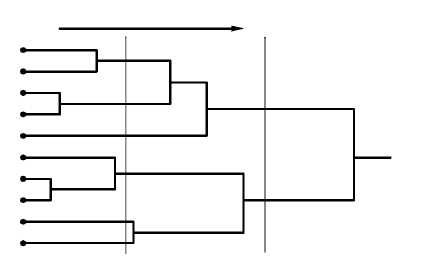
\includegraphics{img/dendrogram.png}
\end{figure}

Na základě dendrogramu se můžeme rozhodnout, kde shlukování zastavíme, udělat tam svislou čáru a tím určit počet shluků. Na obrázku máme svislé čáry dvě, jednou vznikne 6 shluků, druhou pouze dva shluky. \textit{Výška} v dendrogramu znázorňuje vzdálenost shluků

Pro tento typ shlukování je zásadní, jak počítáme vzdálenost shluků:
\begin{itemize}
\item \textbf{Single linkage} Vzdálenost shluků je rovna vzdálenosti dvou nejbližších bodů ve shlucích
\item \textbf{Complete linkage} Vzdálenost shluků je rovna vzdálenosti dvou nejvzdálenějších bodů ve shlucích
\item \textbf{Average linkage} Vzdálenost shluků získáme jako průměr vzdáleností všech dvojic bodů
\item \textbf{Centroid} Vzdálenost shluků získáme jako vzdálenost jejich středů
\end{itemize}

Vliv výpočtu vzdáleností shluků je patrný na obrázku níže, kde pracujeme s jednodimenzionálními daty: 2, 12, 16, 25, 29, 45.

\begin{figure}[ht!]
\centering
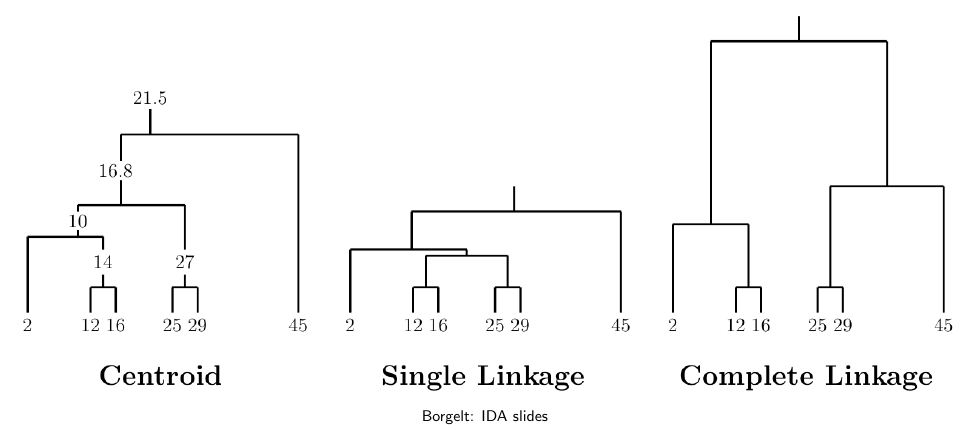
\includegraphics[width=\textwidth]{img/dendrogram-example.png}
\end{figure}

\subsection{Shlukování podle hustoty}

Předpokládáme, že shluky budou mít vyšší hustotu a budou odděleny místy, kde je hustota nižší. Výhodou takového algoritmu je, že nepotřebuje $k$ a umí najít i shluky, které jsou do sebe zamotané, třeba dvě spirály. Naopak problém je, pokud mají shluky různou hustotu.

Shlukování podle hustoty dělá algoritmus DBSCAN. Ten potřebuje dva parametry: velikost okolí a počet sousedů v husté oblasti. Body pak dělí do tří skupin: bod uvnitř shluku (má dost sousedů), hraniční bod (nemá dost sousedů, ale jeho přímí sousedi jsou uvnitř shluku) a bod mimo shluk (nemá dost sousedů, a nesousední s body uvnitř shluku). Výstupem jsou shluky a pak seznam bodů mimo ně.

\subsection{Spektrální shlukování}

Z dat vytvořím síť (graf) a postupně odebírám ty nejdelší hrany. Výsledkem je několik oddělených komponent (shluků). Pro jednoduchost budu pracovat s grafem, ve kterém jsou patrné dvě komponenty (jak se pracuje s body a ne z grafem je popsané níže).

\begin{figure}[ht!]
\centering
\begin{tikzpicture}
    \node[shape=circle,draw=black] (A) at (0,1) {A};
    \node[shape=circle,draw=black] (B) at (0,0) {B};
    \node[shape=circle,draw=black] (C) at (1, 0.5) {C};
    \node[shape=circle,draw=black] (D) at (2.5, 0.5) {D};
    \node[shape=circle,draw=black] (E) at (3.5, 1) {E};
    \node[shape=circle,draw=black] (F) at (3.5, 0) {F} ;

    \draw(A) to (B);
    \draw(B) to (C);
    \draw(A) to (C);
    \draw(D) to (C);
    \draw(D) to (E);
    \draw(D) to (F);
    \draw(E) to (F);   
\end{tikzpicture}
\end{figure}

Nejprve určím matici $S$, kde je jednička, pokud z vrcholu $i$ do vrcholu $j$ vede hrana. Protože je graf neorientovaný, bude matice symetrická. Pokud bychom nepracovali s grafem ale s body, tak matice $S$ bude \textit{similiarity}-matrix, kde počítáme blízkost bodů Gaussovým kernelem (čím bližší body, tím vyšší hodnota) a pak prahujeme podle nějaké konstanty. Tak jako tak vznikne symetrická matice.

Kromě matice $S$ sestavíme taky matici $D$, která bude mít na diagonále stupně vrcholů a jinak bude nulová (tedy je taky diagonální). Z nich spočítáme Laplacián grafu, $L = D - S$.

\begin{equation}
S = 
\left( \begin{array}{cccccc}
0 & 1 & 1 & 0 & 0 & 0\\
1 & 0 & 1 & 0 & 0 & 0\\
1 & 1 & 0 & 1 & 0 & 0\\
0 & 0 & 1 & 0 & 1 & 1\\
0 & 0 & 0 & 1 & 0 & 1\\
0 & 0 & 0 & 1 & 1 & 0\end{array} \right)
%
,
%
D = 
\left( \begin{array}{cccccc}
2 & 0 & 0 & 0 & 0 & 0\\
0 & 2 & 0 & 0 & 0 & 0\\
0 & 0 & 3 & 0 & 0 & 0\\
0 & 0 & 0 & 3 & 0 & 0\\
0 & 0 & 0 & 0 & 2 & 0\\
0 & 0 & 0 & 0 & 0 & 2\end{array} \right)
%
,
%
L = 
\left( \begin{array}{cccccc}
2 & -1 & -1 & 0 & 0 & 0\\
-1 & 2 & -1 & 0 & 0 & 0\\
-1 & -1 & 3 & -1 & 0 & 0\\
0 & 0 & -1 & 3 & -1 & -1\\
0 & 0 & 0 & -1 & 2 & -1\\
0 & 0 & 0 & -1 & -1 & 2\end{array} \right)
\end{equation}

K matici $L$ spočítáme vlastní čísla a vlastní vektory (postup je rozepsaný na webu v QR kódu), a vyjdou čtyři vlastní čísla a vektory:


\begin{figure}[H]
\centering
\begin{minipage}{0.15\textwidth}
\centering
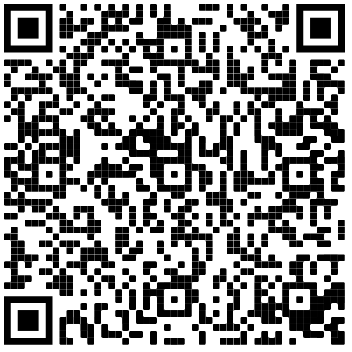
\includegraphics[width=\textwidth]{img/spectral-clustering-qr}
\end{minipage} \hfill
\begin{minipage}{0.84\textwidth}

$\lambda_1 = 0, v_1 = (1, 1, 1, 1, 1, 1)$\\
$\lambda_2 \doteq 0.44, v_2 = (-1, -1, -0.56, 0.56, 1, 1)$\\
$\lambda_3 = 3, v_3 = (-1, 1, 0, 0, 0, 0)$\\
$\lambda_4 \doteq 4.56, v_4 = (-1, -1, 3.56, -3.56, 1, 1)$\\


\end{minipage}
\end{figure}

Teď jsou dva způsoby, jak z toho dostat shluky. Na přednášce jsme si říkali, že vektory dáme jako sloupce do matice $V$, a pak v řádcích té matice máme body. Na ně spustíme nějaké rychlé shlukování, třeba k-means. V přednáškách ze Stanfordu na to jdou ještě lépe, vezmou vektor odpovídající druhému nejmenšímu vlastnímu číslu (to nejmenší je nula a to je nuda), tedy v našem případě $v_2 = (-1, -1, -0.56, 0.56, 1, 1)$. Pak řeknou, že body, kterým přísluší záporné hodnoty (A, B, C) jsou jeden shluk a zbylé body jsou druhý shluk (D, E, F). Pokud chtějí víc clusterů, tak zpracovávají vektor $v_2$, někdy tam je těch úrovní zřetelných víc.


\section{Multivariátní analýza}

\subsection{ANOVA - Analýza rozptylu}

Zjišťujeme, jestli můžeme zamítnout hypotézu $H_0$: průměry ve všech skupinách dat jsou stejné (např. ženy, muži i děti mají stejnou výšku v cm). Mohli bychom to dělat třeba nepárovým t-testem na dvojici vzorků (párový t-test porovnává stejná data před a po, např. náladu lidí před vypitím kafe a po něm). Problém je, že pokud budeme dělat t-test pro každou dvojici skupin, tak to bude časově náročné pro hodně skupin, a taky tam bude víc chyb.

ANOVA předpokládá, že v každé skupině mají data normální rozdělení, že jsou nezávislá, a všechny skupiny mají stejný rozptyl. Zkoumáme vždy právě jednu proměnnou.

Zkusím to na třech třídách dat, $A = \{1, 2, 5\}, B = \{2, 4, 2\}, C = \{2, 3, 4\}$. Nulová hypotéza je, že všechny skupiny mají stejnou střední hodnotu. Všechno v postupu počítáme dvakrát, jednou mezi třídami (between) a pak uvnitř tříd (within). Názvy Ve slidech se to značí treat a error, což mě mátlo, a tak to sem psát nebudu.

Stupně volnosti jsou: $DF_{\text{between}} = k - 1 = 3-1 = 2, DF_{\text{within}} = N - k = 9 - 3 = 6$, kde $N$ je počet datových bodů, a $k$ je počet tříd. Pomocí stupňů volnosti najdeme tabulkovou $F$ hodnotu, $F_{\text{crit}} = 5.14$.

Spočítáme střední hodnota pro skupiny: $\mu_A=2.67,\mu_B=2.67,\mu_C=3$ a celkový průměr $\mu=2.78$. Počítáme \textit{Sum of Squares} ($SS$). Celkový $SS$ je součet vzdáleností všech bodů od střední hodnoty, a má dvě součásti: uvnitř skupiny a mezi skupinami. Sumy nejsou korektně značené, total se počítá pro všechna data, a within pro všechna data, ale odděleně po třídách.

\noindent $SS_\text{total} = \sum (x - \mu)^2 = (1-2.78)^2 + (2-2.78)^2 + (5-2.78)^2 + (2-2.78)^2 + (4-2.78)^2 + (2-2.78)^2 + (2-2.78)^2 + (3-2.78)^2 + (4-2.78)^2  = 13.6$

\noindent $SS_\text{within} = \sum (x - \mu_X) = (1-2.67)^2 + (2-2.67)^2 + (5-2.67)^2 + (2-2.67)^2 + (4-2.67)^2 + (2-2.67)^2 + (2-3)^2 + (3-3)^2 + (3-4)^2 = 13.34$

\noindent $SS_\text{between} = SS_\text{total} - SS_\text{within} = 13.6 - 13.34 = 0.23$

Dál počítáme \textit{rozptyly}:

\noindent $MS_\text{between} = \frac{SS_\text{between}}{DF_text{between}} = \frac{0.23}{2} = 0.12$

\noindent $MS_\text{within} = \frac{SS_\text{within}}{DF_text{within}} = \frac{13.34}{6} = 2.22$

Spočítáme $F$ hodnotu, $F=\frac{MS_\text{between}}{MS_\text{within}} = \frac{0.12}{2.22} = 0.05$

Protože $F<F_\text{crit}$, tedy $0.05 < 5.14$, tak nemůžeme nulovou hypotézu zamítnout, tedy je možné, že všechny skupiny mají stejnou střední hodnotu. F rozdělení je podíl dvou $\chi^2$ rozdělení.

Pokud by ANOVA nulovou hypotézu zamítla, tak pak by se třeba hodilo vědět, která ze skupin má odlišnou střední hodnotu. To nám ale ANOVA říct neumí, a musíme to zjistit jinak, třeba Tukeyho HSD testem. ANOVA umí pracovat pouze s jednou proměnnou, a pracuje s nezávislými měřeními.

\subsection{MANOVA}

Funguje podobně jako ANOVA, ale umožňuje víc náhodných veličin. Předpokladem je, že rozdělení jsou normální a mají napříč třídami stejné kovariační matice, jsou náhodně vzorkované atd, jako u ANOVy. Pro $p$ náhodných veličin vzniknou místo dvou hodnot $SS$ z ANOVy dvě matice $E$ a $H$ z $\mathbb{R}^p$. Pak ve vzorci není $(x - \mu)^2$, ale $(x_i - \mu_i)(x_j - \mu_j)$. Výsledek MANOVY se zpracuje Wilkovým lambda testem (nebo něčím jiným).







\section{Regrese}

\subsection{Lineární regrese}

Chceme data proložit přímkou (nebo rovinou). Předpokládáme, že data jsou lineární a že chyba od dat má normální rozdělení. I přes to, že jsou předpoklady nereálné, to dobře funguje. Pracujeme s modelem $Y = \beta_0 + \beta_1 X + \varepsilon$, kde $\beta$ jsou parametry, které hledáme, a $\varepsilon$ je chyba nebo šum.

Spočítáme RSS (Residual sum of squares) jako součet všech chyb: $RSS = \sum (y_i - \beta_0 - \beta_1x_1)^2$. RSS pak minimalizujeme, abychom dostali optimální parametry $\beta$.

Např. chceme proložit body: $[1, 3], [2,4], [3,5], [4, 4], [5,4], [6,5], [7,6], [8,7]$. Pro jednoduchost přejmenujeme parametry $\beta$, takže pracujeme se vztahem $y = a + bx + \varepsilon$. Vypočítáme $RSS = \sum (y_i - a - bx_i)^2 = (3-a-b)^2 + (4-a-2b)^2 + (5-a-3b)^2 + (4-a-4b)^2 + (4-a-5b)^2 + (5-a-6b)^2 + (6-a-7b)^2 + (7-a-8b)^2 = \cdots = 192 - 76a -370b + 8a^2  + 72ab + 204b^2$.

Tím máme RSS, a to chceme minimalizovat. Nejmenší hodnota bude tam, kde je nulová derivace (tam se křivka zvedá zase zpět nahoru).


\begin{minipage}{0.45\textwidth}
\begin{equation}
\begin{split}
\frac{\partial{RSS}}{\partial{a}} = 0 \\
-76 +16a +72b = 0 \\
16a + 72b = 76 \\
4a + 18b = 19 \\
a = \frac{19 - 18b}{4}
\end{split}
\end{equation}
\end{minipage} \hfill
\begin{minipage}{0.45\textwidth}
\begin{equation}
\begin{split}
\frac{\partial{RSS}}{\partial{b}} = 0 \\
-185+36a+204b=0 \\
36a+204b=185 \\
36\frac{19-18b}{4} + 204b = 185 \\
171 -162b+204b = 185 \\
42b = 14\\
b = \frac{1}{3}\\
a = \frac{19-\frac{18}{3}}{4} = \frac{13}{4}
\end{split}
\end{equation}
\end{minipage}

Dostali jsme parametry přímky: $y = \frac{x}{3} + \frac{13}{4}$. Vyznačené svislé čáry směrem k přímce jsou chyby $\varepsilon$, které jsme minimalizovali.

\begin{figure}[ht!]
\centering
\begin{tikzpicture}
\draw[help lines, color=gray!30, dashed] (0, 0) grid (8.9,8.9);
\draw[->, thick] (-0.2, 0)--(9,0) node[right]{$x$};
\draw[->, thick] (0,-0.2)--(0,9) node[above]{$y$};

\foreach \x/\y in {1/3,2/4,3/5,4/4,5/4,6/5,7/6,8/7}{
	\draw[color=red!60] (\x,\y)--(\x, 13/4+\x/3);
	\node at (\x,\y) {\textbullet};
}

% \foreach \Point in {(1, 3), (2,4), (3,5), (4, 4), (5,4), (6,5), (7,6), (8,7)}{
%     \node at \Point {\textbullet};
% }

\draw (-0.2, 3.183)--(8.9, 6.2167);

\end{tikzpicture}
\end{figure}

Jakmile máme parametry, tak můžeme měřit jejich chybu $SE$ pro každý z parametrů zvlášť, nebo RSE (residual standard error), což je odhad $\sigma$. Z hodnot $SE$ můžeme získat \textit{confidence intervaly}, které nám říkají, že s pravděpodobností $1-\alpha$ bude hodnota parametru ležet uvnitř toho intervalu. $SE(\beta_1)^2 = \frac{\sigma^2}{\sum_{i=1}^m(x_i-\bar{x})^2}$, kde jako $\sigma^2$ můžeme použít odhad $\sigma^2 = \frac{RSS}{m-2}$.

Testování hypotéz: Testujeme $H_0$, že není vztah mezi $X$ a $Y$, tedy $H_0: \beta_1 = 0$. Použijeme t-statistiku: $t = \frac{\beta_1 - 0}{SE(\beta_1)}$, kde za $\beta_1$ dosadíme parametr odhadnutý lineární regresí (a mně se nad něj nechce psát pořád stříšku). Má to $m-2$ stupně volnosti.

K hodnocení přesnosti modelu můžeme použít $R^2$, které nám říká, jaká část rozptylu v datech je vysvětlená modelem. $TSS = \sum_{i=1}^m(y_i - \bar{y})^2$ je celkový součet čtverců (vzdálenost od střední hodnoty), $RSS = \sum_{i=1}^m(y_i - \hat{y}_i)^2$ je vzdálenost bodů od odhadů. Pak $R^2 = \frac{TSS - RSS}{TSS}$.

Pokud chceme pracovat s vícedimenzionálním vstupem, přidáme další parametr beta:  $Y = \beta_0 + \beta_1 X_1 + \beta_2 X_2 + \varepsilon$. Pokud máme pocit, že se různé vstupy ovlivňují, např. zisk v závislosti na reklamu v televizi a reklamu v rozhlase, tak můžeme přidat ještě jeden parametr: $Y = \beta_0 + \beta_1 X_1 + \beta_2 X_2 + \beta_3 (X_1 X_2) + \varepsilon$ a pak zjišťujeme, které $\beta$ je nejvýznamnější.

\paragraph{Ridge regression}
Neminimalizujeme jen $RSS$, ale $RSS + \lambda\sum\beta_i^2$, tedy penalizujeme velká $\beta$, a parametr $\lambda$ určuje, jak přísně. To vede k tomu, že parametry $\beta$ budou co nejnižší, a tedy neužitečné proměnné se skoro nepoužijí ($\beta$ bude nula). Než se na datech spustí ridge regression, je vhodné data standardizovat (ve slidech je na to složitý vzorec, ale předpokládám, že to prostě od dat odečte střední hodnotu, aby byly v průměru na nule). Vhodný parametr $\lambda$ najdeme třeba cross-validací.

\paragraph{Lasso regression} Funguje stejně jako ridge regression, ale minimalizuje $RSS + \lambda\sum|\beta_i|$, tedy ne druhé mocniny. Tím budou koeficienty u neužitečných prediktorů nejen malé, ale dokonce nulové, a budeme je moct úplně zahodit.

\subsection{Nelineární regrese}

\paragraph{Polynomiální regrese} Pracujeme s polynomem nějakého daného stupně (to můžeme určit cross-validací), pak máme $Y = \beta_0 + \beta_1 X + \beta_2 X^2 + \cdots + \varepsilon$ a pokračujeme stejně jako u lineární regrese.

\paragraph{Krokové funkce} Rozdělíme $X$ na menší intervaly a v každém vybereme jako výsledek jednu konstantní hodnotu (třeba střední hodnotu). 

\begin{figure}[ht!]
\centering
\includegraphics[width=0.8\textwidth]{img/splines.png}
\end{figure}

\paragraph{Splines} Rozdělíme $X$ na menší intervaly, hraniční body mezi nimi jsou uzly. Hledáme polynomy takové, aby uvnitř intervalů co nejlépe seděly na datech, a v uzlech měly shodnou hodnotu  (a ideálně i derivaci, aby na sebe navazovaly). Na obrázku jsou ty samé body jako předtím proloženy dvěma parabolami s uzlem v bodě 3.5, a to tak, že v tomto bodě mají stejnou hodnotu a první derivaci.

\begin{figure}[ht!]
\centering
\begin{tikzpicture}
\draw[help lines, color=gray!30, dashed] (0, 0) grid (8.9,9.9);
\draw[->, thick] (-0.2, 0)--(9,0) node[right]{$x$};
\draw[->, thick] (0,-0.2)--(0,10) node[above]{$y$};

\foreach \x/\y in {1/3,2/4,3/5}{
	\draw[color=red!60] (\x,\y)--(\x, {(-0.89 * (\x) ^ 2 + 4.74 *\x + -0.96)});
	\node at (\x,\y) {\textbullet};
}

\foreach \x/\y in {4/4,5/4,6/5,7/6,8/7}{
	\draw[color=red!60] (\x,\y)--(\x, {(0.5 * (\x) ^ 2 + -4.97 *\x + 16)});
	\node at (\x,\y) {\textbullet};
}

\node[color=red] at (3.5, {(0.5 * (3.5) ^ 2 + -4.97 *3.5 + 16)}) {\textbullet};


\draw[color=red!20] plot[domain = 3.5:5] ({\x}, {(-0.89 * (\x) ^ 2 + 4.74 *\x + -0.96)});
\draw[color=red!20] plot[domain = 1.6:3.5] ({\x}, {(0.5 * (\x) ^ 2 + -4.97 *\x + 16)});

\draw plot[domain = 0.8:3.5] ({\x}, {(-0.89 * (\x) ^ 2 + 4.74 *\x + -0.96)});
\draw plot[domain = 3.5:8.2] ({\x}, {(0.5 * (\x) ^ 2 + -4.97 *\x + 16)});


\draw[color=red!60, dashed] (3.5, 0) to (3.5, 9.9);
\node[color=red] at (3.5, {(0.5 * (3.5) ^ 2 + -4.97 *3.5 + 16)}) {\textbullet};

\end{tikzpicture}
\end{figure}

Jak určit, kde budou uzly a kolik jich bude? Můžeme zvolit nějaké $k$ a pak uzly rozmístit rovnoměrně nebo podle kvantilů. Funkce mezi různými uzly můžou být různé - např. uprostřed dat můžeme volit paraboly, a na kraji dat přímky (lineární regresi), aby to bylo na krajích stabilnější (polynomy rychle vyjedou někam pryč). 

\paragraph{Lokální regrese} Hlavní myšlenka je, že ačkoliv data nejsou rozhodně lineární, tak v lokálním měřítku nám lineární odhad bude stačit. Vybíráme jen malé intervaly a na nich děláme po částech normální lineární regresi. Přitom interval nemusí být ostrý - můžeme si vzít nějakou kernel funkci a pomocí ní nějak pravděpodobnostně určovat, nakolik bod do toho \textit{intervalu} patří.


\subsection{Logistická regrese}

Logistická regrese rozděluje data do tříd, nebo přesněji, určuje, s jakou pravděpodobností bod patří do dané třídy. Nejčastěji se dělá pro dvě třídy. Mohlo by se zdát, že stejnou úlohu by zvládla i lineární regrese, ale ta není vhodná - pokud nás zajímá pravděpodobnost, tak bude linreg dávat nesmyslné hodnoty mimo [0, 1], a pokud jsou v datech outlieři, tak se to celé může zvrtnout. Proto do dat nedáváme lineární přímku, ale \textit{sigmoidu}:

\begin{figure}[ht!]
\centering
\begin{tikzpicture}
\draw[help lines, color=gray!30, dashed] (0, 0) grid (10.5,4.5);
\draw[->, thick] (-0.2, 0)--(11,0) node[right]{$x$};
\draw[->, thick] (0,-0.2)--(0,5) node[above]{$y$};

% e = 2.718
\draw[color=red!20] plot[domain = 0:10.3] ({\x}, {4*(2.718 ^ (\x - 5.3)/(1 + (2.718 ^ (\x - 5.3)))});


\draw[color=red!60, dashed] (5.3, 0) to (5.3, 4.5);
\node[color=red] at (5.3, 2) {\textbullet};

\foreach \x in {1, 2, 2.5, 3, 6}{
	\node[Green4] at (\x,0) {\textbullet};
}

\foreach \x in {5, 7, 8, 9, 10}{
	\node[blue] at (\x,4) {\textbullet};
}
\end{tikzpicture}
\end{figure}

Klíčový vztah pro pochopení logistické regrese je poměr pravděpodobností. V angličtině se tomu říká \textit{odds}, tady tomu budu říkat \textit{šance}. Šance je poměr pravděpodobností, že jev nastane vs že nenastane. Pokud se snažím na kostce hodit šestku, je pravděpodobnost úspěchu $p=1/6 \doteq 0.167$ a pravděpodobnost neúspěchu $p = 5/6 \doteq 0.833$. Šance na úspěšný hod je v tomto případě $s = \frac{1/6}{5/6} = 1/5 = 0.2$, ale lépe je to vyjádřit slovně, tedy \textit{jedna ku pěti}.

Nás bude v logistické regresi zajímat, jak se šance mění. To nám ukazuje funkce \textit{logit}, která je vlastně přirozeným logaritmem šancí. Zajímá nás úsek od 0 do 1, kde je funkce rostoucí, v krajních bodech není definovaná a vypadá docela podobně jako tangens. Pokud řekneme, že máme dvě třídy, 0: jev nenastal a 1: jev nastal, které odhadujeme na základě nějakých dat $d$, pak logit svazuje nějakou pravděpodobnost $p$ s hodnotou dat $d$. Praktičtější je inverzní logit, ten nám řekne jaká je pravděpodobnost, že jev nastal, na základě dat $d$. Protože logit nabýval na intervalu (0, 1) hodnoty z $(-\infty, \infty)$, tak inverzní logit je definovaný všude, a to se hodí.

\begin{equation}
\begin{split}
logit(p)=ln(\frac{p}{1-p})\\
log_e(\frac{p}{1-p}) = d\\
\frac{p}{1-p} = e^d\\
p = (1-p)e^d\\
p = \frac{e^d}{1+e^d}\\
P(d) = \frac{e^d}{1+e^d}
\end{split}
\end{equation}

Tím máme funkci $P$, která nám pro pozorovaná data řekne, s jakou pravděpodobností jev nastal. Navíc předpokládáme lineární závislost mezi daty a logaritmem šance (protože to je nejjednodušší a funguje to), tedy $d = ax + b$, kde $x$ je skutečně naměřená hodnota. Pak pravděpodobnost, že při této hodnotě nastal jev, je $P(x) = \frac{e^{ax+b}}{1+e^{ax+b}}$.

Koeficienty $a$ a $b$ najdeme metodou MLE (maximum likelihood estimation), tedy snažíme se vybrat takové parametry, aby naměřená data byla co nejpravděpodobnější. Budeme maximalizovat hodnotu $L$:

\begin{equation}
L(a, b) = \prod_{i, y_i = 1}P(x_i)\cdot\prod_{i, y_i = 0}(1 - P(x_i))
\end{equation}

Pro data výše, kde máme v třídě 0 hodnoty 1, 2, 2.5, 3 a 6 a ve třídě 1 hodnoty 5, 7, 8, 9 a 10, vyjdou nejlépe parametry $a=1, b=-5.3$. Tomu odpovídá funkce $P$ nakreslená v grafu červeně. Hraniční bod v této situaci je 5.3 - hodnoty vyšší než 5.3 pravděpodobně patří do třídy 1, ostatní do třídy 0. Model se dá taky použít ke zjištění, s jakou pravděpodobností patří bod do třídy. Třeba bod 7 patří do třídy 1 s pravděpodobností $P(7) = \frac{e ^{(7 - 5.3)}}{(1 + (e ^{(7 - 5.3))})} = 0.845$.

Logistická regrese jde dál upravit, aby pracovala s více než dvěma třídami, ale to tu ukazovat nebudu.


\subsection{Discriminant Analysis (LDA, QDA)}

Separuje datové třídy tím, že najde \textit{discriminant score} $\delta$, které se počítá z parametrů (Gaussovských) rozdělení. Vznikne rozhodovací hranice, která je buď přímkou (pak šlo o LDA, linear discriminant analysis), nebo křivkou (pak šlo o QDA, quadratic discriminant analysis).

\begin{figure}[ht!]
\centering
\includegraphics[width=0.7\textwidth]{img/lda-qda.jpg}
\end{figure}

Diskriminant je $\delta_k(x) = x\frac{\mu_k}{\sigma^2} - \frac{\mu_k^2}{2\sigma^2} + log(\pi_k)$, kde $\sigma_k$ je směrodatná odchylka ve třídě $k$, $\mu_k$ je střední hodnota ve třídě $k$, a $\pi_k$ je pravděpodobnost výskytu třídy $k$ v datech. Funguje to i na víc než 2 třídách, pak musí mít společnou kovariační matici.

Pravděpodobnost získáme z diskriminantu jako $P(Y=k|X=x) = \frac{e^{\delta_k(x)}}{\sum_{l=1}e^k{\delta_k(x)}}$. LDA funguje dobře, pokud máme málo dat a data jsou dobře separovatelná.



















\end{document}

\chapter[Zajištění kvality software]{B4M36ZKS \\[1ex]\Large{Metodika testování software. Metody vytváření testů z modelu aplikace. Automatické testování}}

%\chapter[Bezpečnost systémů]{B4M36BSY \\[1ex]\Large{Bezpečnostní analýza operačních systémů, bezpečný vývoj software a bezpečnost webových aplikací. Analýza útoků a škodlivého kódu. Bezpečnost mobilních zařízení.}}

Bezpečnost má tři části, říká se jim CIA:
\begin{description}
\item[Confidentiality] Služba nesmí odhalit soukromá data
\item[Integrity] Data nesmí jít změnit 
\item[Availability] Služba musí být stabilní a dostupná
\end{description}

Návrh systému - nejprve navrhneme směrnice (policies), tj pravidla, která chceme dodržovat. Směrnice určují, kdo má k čemu přístup, kdo může co dělat atd. Pokud jsou směrnice správně navržené, pak by měl být systém bezpečný. Navrhnout správnou směrnici je těžké - např. Amazon umožňoval komukoliv přidat k účtu další kreditní kartu bez jakéhokoliv ověření identity, a pak umožňoval na základě znalosti čísla jedné karty zjistit část čísla jiné karty, což je špatně.




\section{Bezpečný vývoj software}

Začínáme tím, že si ujasníme, co to je za aplikaci, co má dělat a pro koho má být (tedy funkcionalita). Pak je potřeba vědět, z jaké strany přijde útok, jak závažné ty útoky můžou být (což je hrozně těžké odhadnout). A na základě toho se pak určíme, jestli a jak se budeme bránit - někdy je prostě nejjednodušší nedělat nic, protože dopad je malý a prevence je drahá.

Aplikaci naplánujeme, nakreslíme si diagram, a pak se snažíme najít všechny možné způsoby, jak na to půjde útočit (hrozby). Ty jsou dělené do šesti tříd - STRIDE:
\begin{description}
\item[Spoofing] Manipulace, např. s identitou (říkám, že jsem někdo jiný)
\item[Tampering] Manipulace s daty nebo s kódem
\item[Repudiation] Popření toho, že se něco stalo (např. můžu tvrdit e-shopu, že mi to ještě nedorazilo, ačkoliv už mám zboží doma)
\item[Information disclosure] Únik informací (přečtu něco, co by mi nemělo být viditlené)
\item[Denial of service] Zablokování služby
\item[Escalation of privilege] Zvýšení práv (dělám víc, než by můj účet měl mít možnost dělat)
\end{description}

Hrozby taky můžeme sepsat do \textit{attack tree}, což je sekvence akcí, které může útočnik dělat, a co tím může získat. Hrozby pak nějak ohodnotím, což je ale těžké - zajímá nás, s jakou pravděpodobností útok nastane, kolik bude stát prevence, kolik bude stát oprava následků, a my žádné z těchto čísel neumíme určit.

K tomu se vytvořily metody hodnocení, třeba DREAD od Microsoftu. Tam se v každé kategorii dává skóre na škále od 0 do 10:
\begin{description}
\item[Damage] Jak velká je škoda?
\item[Reproducibility] Jak složité je ten útok zopakovat?
\item[Exploitability] Jak zkušený musí útočník být?
\item[Affected users] Na kolik uživatelů to dopadne?
\item[Discoverability] Jak složité je to pro útočníka najít?
\end{description}

\noindent Na základě hodnocení se rozhodneme, co uděláme s každou hrozbou:
\begin{itemize}
\item Neuděláme nic, protože škoda je malá a oprava by byla drahá
\item Komponentu smažeme, protože je extra děravá, a stejně to nikdo nepoužívá
\item Opravíme to
\end{itemize}

Celkově je při vývoji vhodné kontrolovat kód (motivuje to lidi, aby ho psali hezky), spouštět appku s co nejmenšími právy (když se to vysype, bude menší škoda), mít bezpečné výchozí nastavení (většina uživatelů to nechce vůbec řešit), mělo by to být pohodlné, protože jinak to lidi začnou obcházet (místo firewallu se připojí z mobilu, do hesla si dají counter protože má být složité a často měněné), důkladně testovat, nemíchat kód a data (to dělá bordej v XSS, SQLi atd).



\section{Postranní kanály}

Dva procesy (třeba ve virtuálních strojích) chtějí komunikovat, a vuyžívají datové kanály, které nejsou určeny k přenosu dat. To je problém, protože nemůžeme kontrolovat, že vše odpovídá směrnici. Jsou dva druhy:
\begin{itemize}
\item Storage: Dokážeme něco změnit, třeba bit v metadatech, a na základě toho přenášet informaci (např. dva procesy sdílejí disk a mohou nastavit, kde zastaví čtecí hlava, a tím komunikovat)
\item Timing: Dokážeme manipulovat, jak dlouho něco trvá, a tím přenášet informaci 
\end{itemize}

Postranní kanály nejde nikdy úplně odstranit. Ale přenesou jen malé množství dat, takže se dá třeba říct, že se chceme zbavit všech postranních kanálů, které mají větší kapacitu než 1bit za sekundu. Kanály mohou být se šumem nebo bez, ale i když tam je šum, tak se ho můžeme zbavit nějakým kódováním, i když tím ztratíme rychlost přenosu.


\subsection{Útoky na postranní kanály}

Útočník přistupuje ke službě a chce z ní vytáhnout nějaká data. Využívá toho, že služba se chová různě (různě se větví), podle toho, jaká data do ní dáme. Např. funkce kontroluje uživatelovo heslo, a vrátí \texttt{False} hned, jakmile narazí na špatné písmenko. Pak můžeme jednoduše hádat hesla tak, že vyzkoušíme všechna možná jednoznaková hesla, a jedno z nich bude trvat déle - to je to, ve kterém se začal porovnávat i další znak, a to je to, ve kterém máme správný  první znak. To rapidně zjednodušuje hádání hesel, pro desetiznakové heslo byla složitost $27^{10}$ a teď je $27\cdot 10$.

Kromě časových útoků jsou i útoky na spotřebu (čipové karty), na zvuk, chybové hlášky, odraz monitoru na zeď za uživatelem atd. Postranní útoky se těžko hledají - je to jeden z důvodů, proč se silně nedoporučuje implementovat si vlastní kryptografii. 

\paragraph{Steganografie} Posíláme tajná data tak, aby nikdo nevěděl, že je vůbec posíláme. Např. vytetované pod vlasy otroků, v least significant bitu v barvách obrázku, mrkání na videu (zpráva "torture" během vietnamské války).




\section{Modely řízení přístupu}

Matice přístupu je tabulka, ve které jsou zdroje (např. soubory) a kdo (procesy, uživatelé) k nim má jaký přístup.

\paragraph{Discretional Access Control (DAC)} Je metoda řízení přístupu na Unixu, soubor má vlastníka a daná práva pro čtení/zápis/spouštění pro vlastníka, skupinu a ostatní. Vznikl, když počítače začaly mít víc uživatelů, a ti si chtěli být jistí, že si omylem navzájem nesmažou data. Nevýhodou je, že když uživatel spustí program, tak ten program běží s právy toho uživatele. Druhou nevýhodou je, že ve velkých firmách to neumožňuje dostatečnou kontrolu. Další nevýhodou je, že vlastník souboru může přístupová práva ostatních měnit, to se nehodí zejména v armádě. Používá se spíš z historickou kontrolou.

\paragraph{Access Control list} Každý zdroj má majitele, a majitel může se zdrojem dělat nějaké činnosti dle seznamu. DAC se na pozadí implementuje jako tenhle seznam.

\paragraph{Tokeny} Konkurentem pro ACL jsou tokeny, kde každý zdroj dá přístup (nebo jiné právo) každému, kdo má správný token. Vlastností tokenů je, že si je uživatelé mohou předávat a někomu tak věnovat přístup.

\paragraph{Mandatory Access Control} vzniklo jako náhrada DAC pro armádu. Kontrolu nad právy nemají vlastníci souborů, ale někdo centrální. V armádě (USA) jsou různé úrovně tajnosti:

\begin{itemize}
\item \textbf{Unclassified}
\item \textbf{Classified}
\item \textbf{Secret} - pokud toto unikne, způsobí to ztrátu několika životů
\item \textbf{Top Secret} - pokud toto unikne, způsobí to ztrátu mnoha životů
\end{itemize}

Chceme zajistit, aby tajné dokumenty nemohl číst někdo, kdo na to nemá právo. Druhé omezení se týká zápisu: uživatelé, kteří mají přístup na úrovni Top Secret, budou vytvářet pouze soubory na úrovni Top Secret (tedy nikdo pod nimi si to nepřečte). To je tam proto, aby nešly vynášet přísně tajné informace.

Je to dost těžké naimplementovat, protože systém má současně otevřeno víc souborů, a pokud je jeden z nich top secret, tak by se měly všechny nastavit jako top secret. Jednodušší je to dělat přes virtuální stroje, kde každý běží na jedné bezpečnostní úrovni, a mohou komunikovat (posílat si soubory) přes hlídané kanály.

\paragraph{SE (Security Enhanced) Linux} Zdroje a spotřebitelé mají značky (labels). Spotřebitel může použít zdroj jen tehdy, pokud má správnou značku. Tím lze zajistit to, že zlý proces, ačkoliv běží s právy uživatele, nemůže napáchat žádnou škodu.

\paragraph{Role-based} je systém, který se víc hodí ve firmách. Přístup se povoluje na základě role - zaměstnanec na pozici sekretářky má přístup jinam, než zaměstnanec na pozici programátora. Je to podobné jako skupiny na Unixu, ale Unix umožňuje, aby jeden uživatel byl ve více skupinách.






\section{Operační systémy}






















\documentclass[10pt,a4paper]{article}
\usepackage[utf8]{inputenc}
\usepackage[czech]{babel}
\usepackage[T1]{fontenc}
\usepackage{amsmath}
\usepackage{amsfonts}
\usepackage{amssymb}
\usepackage{delarray}

% graphs
\usepackage{tikz}
\usetikzlibrary[topaths]

\usepackage[left=2cm,right=2cm,top=2cm,bottom=2cm]{geometry}
\title{B4M01MKR - Symetrická a asymetrická kryptografie. Základní kryptosystémy. Faktorisace čísel. Hashování.}
\date{}
\begin{document}
\maketitle
\section{Symetrická a asymetrická kryptografie}
Symetrická a asymetrická kryptografie se liší vlastnostmi a způsobem použití klíčů. Zatímco v symetrické kryptografii používají obě komunikující strany stejný klíč, u asymetrické kryptografie jsou klíče dva: soukromý klíč (často značený $d$), a veřejný klíč (často značený $e$).

Symetrická kryptografie je rychlejší a proto se používá pro většinu komunikace, ale vyžaduje bezpečnou výměnu klíče. Asymetrická kryptografie je pomalejší, a podle použití klíčů umožňuje dvě věci:
\begin{itemize}
\item Kdokoliv může zašifrovat zprávu veřejným klíčem, a zprávu si pak může přečíst jen ten, komu je určena (majitel soukromého klíče)
\item Majitel klíče pošle zprávu a k ní hash zašifrovaný soukromým klíčem. Takovou zprávu si může kdokoliv přečíst, ale zprávu nelze zfalšovat (je jasné, že autorem může být jedině majitel klíče).
\end{itemize}

Díky tomu mohla vzniknout hierarchie certifikačních autorit a certifikátů. Uživatel může ověřit (podle certifikační autority, které věří), že server na druhé straně komunikace se za nikoho nevydává, a skutečně jde třeba o webovou stránku banky. S použitím asymetrické kryptografie si uživatel se serverem vymění hesla a dál mohou používat rychlejší symetrickou kryptografii.

\section{Matematika používaná v kryptografii}
\subsection{Dělitelnost, modulo, rovnice}

Základní věta aritmetiky: Každé přirozené číslo $n$ jde zapsat jako jednoznačný součin prvočísel, kde \textbf{prvočíslo} je číslo, které je dělitelné jen jedničkou a sebou samým.

\subsubsection{Počítání modulo}

\textbf{Dělení se zbytkem}: $\forall a, b \in \mathbb{Z}, a, b > 0, \exists q, r \in \mathbb{Z},$ že $ a = qb + r$, a přitom $0 \leq r \le b$, a $q, r$ jsou jednoznačné. Když je $r$ (zbytek) nulový, řekneme, že $a$ je dělitelné $b$ nebo že $b$ dělí $a$, značíme $b \mid a$. Relace dělitelnosti na $\mathbb{Z}$ je reflexivní, tranzitivní a antisymetrická, dá se znázornit Hasseho diagramem (Obrázek \ref{fig:hasse}).

\begin{figure}[h!]
\label{fig:hasse}
\centering
\begin{tikzpicture}
    \node (12) at (0,0) {12};
    \node (4) at (-1, -1) {4};
    \node (6) at (1, -1) {6};
    \node (2) at (-1, -2.5) {2};
    \node (3) at (1, -2.5) {3};
    \node (1) at (0, -3.5) {1} ;

    \path  (12) edge node {} (4);
    \path  (12) edge node {} (6);
    \path  (6) edge node {} (2);
    \path  (6) edge node {} (3);
    \path  (4) edge node {} (2);
    \path  (1) edge node {} (2);
    \path  (1) edge node {} (3);
\end{tikzpicture}
\caption{Hasseho diagram pro číslo 12}
\end{figure}

\textbf{Největší společný dělitel (GCD)} dvou čísel $a, b$ (značíme $gcd(a,b)$) je takové číslo $d$, kde:
\begin{itemize}
\item $d \mid a \wedge d \mid b$
\item $d$ je dělitelné všemi společnými děliteli obou čísel
\item $d \geq 0$
\end{itemize}
V Hasseho diagramu najdeme GCD dvou čísel jako první číslo, ve kterém se můžeme sejít při cestě dolů - pro čísla 4 a 6 jde o číslo 2.

\textbf{Nejmenší společný násobek (LCM)} čísel $a, b$ (značíme $lcm(a, b)$) je nejmenší takové $d$, které je dělitelné číslem $a$ a zároveň je dělitelné číslem $b$. V Hasseho diagramu najdeme LCM jako první číslo, ve kterém se můžeme sejít při cestě nahoru - pro čísla 3 a 4 je LCM 12.

Máme nějaké $n \in \mathbb{N}$, pak čísla $a, b \in \mathbb{Z}$ jsou \textbf{kongruentní modulo} $n$, pokud $n \mid (b-a)$. Kongruence se značí $a \equiv b\mod n$, je to ekvivalence a rozdělí celá čísla na $n$ tříd, kde všechny prvky ve třídě mají stejný zbytek po dělení číslem $n$. Přirozená čísla rozdělená na třídy ekvivalence podle $n$ značíme $\mathbb{Z}_n$. Relace kongruence je zachovaná při sčítání i násobení.

Například můžeme celá čísla rodělit podle $\mathbb{Z}_4$:
\begin{itemize}
\item ${-4, 0, 4, ...} \equiv  0$
\item ${-3, 1, 5, ...} \equiv  1$
\item ${-2, 2, 6, ...} \equiv  2$
\item ${-1, 3, 7, ...} \equiv  3$
\end{itemize}

A kongruence je zachovaná i při násobení a sčítání:

\begin{itemize}
\item $-4 \times 3 = -12 = 0$, nebo $-4 \times 3 = 0 \times 3 = 0$ 
\item $-4 + 3 = -1 = 3$, nebo $-4 + 3 = 0 + 3 = 3$ 
\end{itemize}

\subsubsection{Euklidův algoritmus}
\textbf{Euklidův algoritmus} umožňuje v lineárním čase najít $gcd(a,b)$. Dělá to tak, že rozkládá $a$ jako $a = qb + r$, a dokud je zbytek $r$ nenulový, rekurzivně spouští $gcd(b,r)$. Výhodné je použít místo tohoto postupu výpočet přes úpravy matic, kde dostaneme navíc koeficienty pro Bezoutovu větu.

\textbf{Př.:} Euklidovým algoritmem chceme najít $gcd(260, 84)$.

\begin{center}
\begin{tikzpicture};
    \node (A) at (0, 0) {$gcd(260, 84) = 4$};
    \node (B) at (0, -1) {$260 = 3 \cdot 84 + 8$};
    \node (C) at (0, -2) {$84 = 10 \cdot 8 + 4$};
    \node (D) at (0, -3) {$8 = 2 \cdot 4 + 0$};
    
    \draw[->](-0.4,-0.2) to[out=270,in=90] (-1,-0.8);
   	 \draw[->] (0.25,-0.2) to[out=270,in=90] (0.4,-0.8);
   	 
    \draw[->](0.4,-1.2) to[out=270,in=90] (-1,-1.8);
   	 \draw[->] (1.1,-1.2) to[out=270,in=90] (0.4,-1.8);
   	 
    \draw[->](0.4,-2.2) to[out=270,in=90] (-0.8,-2.8);
   	 \draw[->] (1,-2.2) to[out=270,in=90] (0.25,-2.8);
   	 
   	 \draw (0.25,-3.2) to[out=270,in=180] (1.5, -3.7);
   	 \draw[->] (1.5, -3.7) to[out=0,in=0] (1.3, 0);
\end{tikzpicture}
\end{center}

\textit{Jakmile získáme $r = 0$, tak víme, že hodnota GCD je uložena v $b$. V tomto případě $gcd(260, 84) = 4$.}

\textbf{Př.:} Chceme najít $gcd(260, 84)$ maticově.

\[ \left( \begin{array}{cc|c}
1 & 0 & 260\\
0 & 1 & 84
\end{array} \right)
%
\sim
%
\left( \begin{array}{cc|c}
1 & -3 & 8\\
0 & 1 & 84
\end{array} \right)
%
\sim
%
\left( \begin{array}{cc|c}
1 & -3 & 8\\
-10 & 31 & 4
\end{array} \right)
%
\sim
%
\left( \begin{array}{cc|c}
21 & -65 & 0\\
-10 & 31 & 4
\end{array} \right)
\]

\textit{Maticové řešení je podrobněji popsané níže u diofantických rovnic. Kromě toho, že jsme našli řešení, máme i jiné užitečné vztahy, a sice vyjádření nuly: $21 \cdot 260 - 65 \cdot 84 = 0$ a vyjádření GCD: $-10 \cdot 260 + 31 \cdot 84 = 4$. Maticový výpočet se hodí, když hledáme GCD více čísel najednou:}

\[ \left( \begin{array}{ccc|c}
1 & 0 & 0 & 90\\
0 & 1 & 0 &  78\\
0 & 0 & 1 &  72
\end{array} \right)
%
\sim
%
\left( \begin{array}{ccc|c}
1 & 0 & -1 & 18\\
0 & 1 & -1 &  6\\
0 & 0 & 1 &  72
\end{array} \right)
%
\sim
%
\left( \begin{array}{ccc|c}
1 & -3 & 2 & 0\\
0 & 1 & -1 &  6\\
0 & -12 & 13 &  0
\end{array} \right)
\]

\[ \left( \begin{array}{ccc|c}
1 & 0 & 0 & 70\\
0 & 1 & 0 &  110\\
0 & 0 & 1 &  154
\end{array} \right)
%
\sim
%
\left( \begin{array}{ccc|c}
1 & 0 & 0 & 70\\
-1 & 1 & 0 &  40\\
-2 & 0 & 1 &  14
\end{array} \right)
%
\sim
%
\left( \begin{array}{ccc|c}
11 & 0 & -5 & 0\\
5 & 1 & -3 &  -2\\
-2 & 0 & 1 &  14
\end{array} \right)
%
\sim
%
\left( \begin{array}{ccc|c}
11 & 0 & -5 & 0\\
-5 & -1 & 3 &  2\\
33 & 7 & -20 &  0
\end{array} \right)
\]

\subsubsection{Bezoutova věta}
\textbf{Bezoutova věta} říká, že největší společný dělitel jde zapsat jako vztah $a,b$, tedy: $gcd(a, b) = sa + tb$, kde $s,t$ jsou celá čísla.

\subsubsection{Diofantické rovnice}
\textbf{Diofantická rovnice} je rovnice ve tvaru $ax + by = c$, kde $a,b,c \in \mathbb{Z}$. Diofantická rovnice má řešení, právě když $gcd(a,b) \mid c$. Řešení má partikulární a homogenní část.

\textbf{Př.:} V $\mathbb{Z}_{45}$ chceme řešit rovnici $12x = 6$.

\textit{Rovnici si nejprve převedeme na diofantickou, tj dostaneme $12x + 45y = 6$. Vyrobíme si jednotkovou matici o dvou sloupcích, kde první sloupec odpovídá neznámé $x$ a druhý sloupec neznámé $y$. Příslušné hodnoty v rovnici napíšeme do pravého sloupce a matici upravíme.}
\[ \left( \begin{array}{cc|c}
1 & 0 & 12\\
0 & 1 & 45
\end{array} \right)
%
\sim
%
\left( \begin{array}{cc|c}
1 & 0 & 12\\
-4 & 1 & -3
\end{array} \right)
%
\sim
%
\left( \begin{array}{cc|c}
-15 & 4 & 0\\
-4 & 1 & -3
\end{array} \right)
\]
\textit{Úpravy skončí, když se v pravém sloupci objeví nula. Druhá hodnota je největší společný dělitel čísel 12 a 45, po přenásobení řádku $-1$ vidíme, že $gcd(12,45)=3$. Protože $3 \mid 6$, bude mít diofantická rovnice řešení.}

\textit{Máme homogenní řešení $12\times(-15) + 45\times 4 = 0$ a partikulární řešení $12\times4 + 45\times(-1) = 3$. Druhou rovnici ale musíme vynásobit dvěma, abychom dostali na pravé straně 6 (odtud požadavek, aby $3\mid6$), tím dostaneme partikulární řešení $12\times8 + 45\times(-2) = 6$. Řešení se zapisuje ve tvaru $(x,y) = (x_p,y_p) + k(x_0,y_0)$, a řešení diofantické rovnice je $(x,y) = (8, -2) + k(-15,4)$. V zadání jsme ale měli řešit pouze rovnici pro $x$, a tak výsledek je $x = 8 - 15k$.}

\subsection{Grupy}
Máme množinu $A$ a operaci $\cdot$~. Dvojice $(A,\cdot)$ je grupa, pokud:
\begin{itemize}
\item Platí asociativita, tj $x\cdot(y\cdot z) = (x\cdot y)\cdot z$
\item Existuje neutrální prvek $e \in A$ (jednotka), pro který platí, že $\forall x \in A: e\cdot x = x = x \cdot e$.
\item Všechny prvky mají inverze, tj $\forall x ~\exists y: x\cdot y = e = y \cdot x$.
\end{itemize}
Řekneme, že $(A,\cdot)$ je Abelova grupa, když je navíc operace $\cdot$ komutativní, tedy $x\cdot y = y \cdot x$.
Dvojice $(\mathbb{Z}, +)$,  $(\mathbb{R}^+, \times)$,  $(\mathbb{Z}_n, +)$ jsou grupy. $(\mathbb{Z}_n^*, \times)$, kde $\mathbb{Z}_n^*$ je podmnožina prvků ze $\mathbb{Z}_n$ nesoudělných s $n$, je taky grupa.

\textbf{Řád grupy} je počet prvků v $A$. Grupy mohou být konečné i nekonečné.

V grupách $\mathbb{Z}_n^*$ jsou všechna čísla menší než $n$, která jsou s $n$ nesoudělná. Počet nesoudělných čísel, a tedy i řád grupy, vyjařuje \textbf{Eulerova funkce} $\varphi(n)$.
\begin{itemize}
\item $\varphi(p) = p-1$ pro prvočíslo $p$.
\item $\varphi(p^k) = p^k - p^{k-1} = p^{k-1}(p-1)$ pro $k$-tou mocninu prvočísla $p$.
\item $\varphi(n\cdot m) = \varphi(n)\cdot\varphi(m)$ pro nesoudělná čísla $m,n$.
\end{itemize}

Nejmenší $m$ takové, že $\forall a \in G: a^m = 0$ se nazývá \textbf{exponent grupy}. Exponent grupy $\mathbb{Z}_n^*$ lze spočítat \textbf{Carmichaelovou fcí} $\lambda(n)$.
\begin{itemize}
\item $\lambda(\prod_{i=1}^r p_i^{e_i}) = lcm\{\lambda(p_1^{e_1}), \ldots, \lambda(p_r^{e_r})\}$ pro složené číslo.
\item $\lambda(p^e) = \varphi(p^e) = p^e - p^{e-1} = p^{e-1}(p-1)$ pro $e$-tou mocninu prvočísla $p$, kde $p > 2$.
\item $\lambda(2^e) = \frac{\varphi(2^e)}{2} = 2^{e - 2}$ pro mocninu dvojky, kde $e \geq 3$.
\item $\lambda(4) = 2$
\item $\lambda(2) = 1$
\end{itemize}

\subsubsection{Cyklické grupy}

Nechť $(G,\cdot)$ je grupa s neutrálem 1, $a \in G$. Nejmenší $r \in \mathbb{N}$ takové, že $a^r = 1$ v $G$ se nazývá \textbf{řád prvku} $a$, značí se $r(a)$. Pokud takové číslo neexistuje, je řád nekonečný.

Pro prvek $a \in G$ je množina $P = \{a^i~|~i = 1 \ldots r(a)\}$ \textbf{cyklickou podgrupou} grupy $G$. Cyklickou podgrupu generovanou prvkem $a$ značíme $\langle a \rangle$. Pokud pro nějaký prvek $a \in G$ platí $\langle a \rangle  = G$, pak řekneme, že grupa $G$ je \textbf{cyklická} a prvek $a$ je její \textbf{generátor}.

Grupy $(\mathbb{Z}, +)$ a $(\mathbb{Z}_n, +)$ jsou cyklické a jejich generátorem je např. prvek 1. Grupy $(\mathbb{Z}_n^*, \times)$ jsou cyklické pro $n$ prvočíslo, mocninu prvočísla, nebo $n$ ve tvaru $2p^e$ pro liché prvočíslo $p$.

Cyklické grupy jsou specifické tím, že mají jasné velikosti podgrup a od každé velikosti existuje jen jedna podgrupa.

\subsection{Euler-Fermatova věta}
Nechť $(G,\cdot)$ je konečná grupa s neutrálem 1. Pak $\forall a \in G: a^{|G|} = a\cdot a\cdot a\cdots a = 1$ v $G$.

To nám říká, že když umocníme na velikost grupy, dostaneme jednotku. 
Euler-Fermatova věta se používá při počítání velkých mocnin, protože umožňuje zmenšit exponent.

\subsection{Algoritmus opakovaných čtverců}
Algoritmus opakovaných čtverců taky zrychluje počítání mocnin. Fungování je nejlépe vidět na příkladu, spočítáme $5^{17}$ v $\mathbb{Z}_{27}$.
\begin{enumerate}
\item Exponent napíšeme jako binární číslo:\\ $17 = 16 + 1 = 10001_{bin}$
\item Do mezer mezi cifry vložíme znak $S$, nuly smažeme, jedničky nahradíme znakem $X$:\\ $10001 = 1S0S0S0S1 = 1SSSS1 = XSSSSX$.
\item Začneme s číslem 1 a postupně zpracováváme znaky $S$ a $X$. Po přečtení znaku $S$ mezivýsledek umocníme na druhou, po přečtení znaku $X$ mezivýsledek vynásobíme základem. Přitom pořád si mezivýsledek udržujeme v modulu $n$:\\ $1XSSSSX \rightarrow 5SSSSX \rightarrow 25SSSX = -2SSSX \rightarrow 4SSX \rightarrow 16SX \rightarrow 256X = 13X \rightarrow 65 = 11$ v $\mathbb{Z}_{27}$.
\end{enumerate}

\subsection{Čínská věta o zbytcích}
Díky čínské větě umíme řešit soustavy rovnic. Mějme po dvou nesoudělná přirozená čísla $n_1, \ldots, n_k$ a k nim libovolná přirozená čísla $a_1,\ldots,a_k$. Pak soustava rovnic $x_i \equiv a_i \mod n_i, i = 1,\ldots,k$ má právě jedno řešení modulo $n = \prod_{i=1}^{k}n_i$.

Řešení se najde tak, že pro každou rovnici najdeme takové $q_i$, aby platil vztah $q_i \equiv 1 \mod q_i$ a zároveň $q_i \equiv 0 \mod q_j, j \neq i$ (tedy $q_i$ je nulové ve všech modulech vyjma svého vlastního, kde má hodnotu jedna).

Takové $q_i$ můžeme najít tak, že vynásobíme všechny moduly (vyjma $n_i$), výsledek označme $m_i$, a najdeme nějaké $t_i$ tak, aby $m_iq_i \equiv 1 \mod n_i$. Tato soustava určitě bude mít řešení, protože $n_i$ jsou nesoudělná.

Řešení soustavy pak je $x = \sum_{i=1}^{k}q_ia_i$.

Př.: Řešte soustavu: $x \equiv 2 \mod 4$, $x \equiv 0 \mod 5$, $x \equiv 1 \mod 9$, $x \equiv 2 \mod 11$.

Spočítáme koeficient $q$ pro modul 4. $q_4 = 5\cdot9\cdot11\cdot t = 495t$. Chceme, aby $495t \equiv 1 \mod 4$, což si můžeme ještě upravit na $3t \equiv 1 \mod 4$. Vidíme, že vhodné $t$ je 3, protože $3\times 3 = 9 \equiv 1 \mod 4$. Dosazením hodnoty $t$ dostaneme $q_4 = 495t = 495 \times 3 = 1485$. Obdobně dostaneme $q_5 = 396$, $q_9 = 1540$, $q_{11} = 540$.

Z koeficientů dostaneme výsledek: $x = 2q_4 + 0q_5 + 1q_9 + 2q_{11} = 2970 + 0 + 1540 + 540 = 5590$. Ale my pracujeme modulo $n = 4\cdot5\cdot9\cdot11 = 1980$, proto je výsledek $x = 5590 \equiv 3610 \equiv 1630 \mod 1980$.

\section{Generování prvočísel}
Generování prvočísel zjednodušeně probíhá tak, že se (chytře) generují čísla, a následně se ověřuje, jestli vzniklo prvočíslo. Testy prvočíselnosti můžeme dělat deterministicky nebo pravděpodobnostně. Deterministické testy zmíníme jen okrajově:

\begin{itemize}
\item \textbf{Hrubou silou}: Dělíme $n$ všemi (prvo)čísly až do $\sqrt{n}$ a tím vyloučíme dělitelnost. Složitost takového postupu je $O(2^{0.5\cdot len(n)}\cdot len(n))$
\item \textbf{Agrawal, Kayal, Saxena (AKS)}:  test prvočíselnosti je sice polynomiální a deterministický, ale jeho složitost je $O(len(n)^{10.5 + o(1)})$
\end{itemize}

Pravděpodobnostní testy mají jednostrannou chybu. Pokud odpoví, že číslo je \texttt{složené}, je to vždy pravda. Odpověď \texttt{prvočíslo} ale správná být nemusí - mohlo se stát, že test důkaz o složenosti "přehlédl". Ve vstupu testu je testované číslo a nějaký svědek. Na základě jednoho svědka algoritmus rozhodne. Pro získání požadované spolehlivosti se test několikrát opakuje s různými svědky.

\subsection{Fermatův test}
Fermatův test zavádí pro testované $n$ množinu svědků prvočíselnosti $K_n$, ve které jsou ty prvky, které po umocnění na $n-1$ vrátí jedničku.

 Pokud je $n$ prvočíslo, pak $K_n$ je shodná s $\mathbb{Z}_n^*$. Pokud $n$ prvočíslo není, pak rozdělíme $\mathbb{Z}_n^*$ na třídy (podgrupy). Počet tříd $k$ nutně dělí velikost grupy.
\begin{itemize}
\item Pro $k = 1$ nastává výjimečná situace, totiž že $|\mathbb{Z}_n^*| = |K_n|$. Takové složené $n$ se nazývá Carmichaelovo a platí pro něj, že $a^{n-1} = 1 \mod n$ pro libovolné $a$. Fermatův test nedokáže rozpoznat Carmichaelova čísla jako složená.
\item Pro $k \geq 2$ platí, že  $|K_n| = \frac{1}{k}|\mathbb{Z}_n^*|$.  Obecně můžeme říct, že $|K_n| \leq \frac{1}{2}|\mathbb{Z}_n^*|$, ale to je hrubý odhad, častěji bude $K_n$ daleko menší.
\end{itemize}

Fermatův test bere na vstupu testované číslo $n$ a svědka $a$.
\begin{verbatim}
fermat-test(n, a):
    b = pow(a, n-1) % n
    if b == 1:
        return "asi prvočíslo"
    else:
        return "určitě složené"
\end{verbatim}

\textbf{Př.:} Fermatovým testem ověřte, zda 21 je prvočíslo. Použijte svědky 8, 6 a 2.
\begin{itemize}
\item \texttt{fermat-test(21, 8) = "asi prvočíslo"}, protože $8^{20} = \cdots = 1 \mod 21$.  Pravděpodobnost chyby je nejvýš 1/2. Pokud bychom si to spočítali (našli řešení $x^{20} = 1$), uvidíme, že takové $x$ jsou čtyři (1, 8, 13, 20) a zabírají pětinu z celkových 20ti prvků. Pravděpodobnost omylu testu je tedy daleko nižší, a to 1/5.
\item \texttt{fermat-test(21, 6) = "složené"}, protože $6^{20} = \cdots = 15 \neq 1 \mod 21$. Navíc když spočítáme gcd(21, 6) = 3, našli jsme jeden z faktorů.
\item \texttt{fermat-test(21, 2) = "složené"}, protože $6^{20} = \cdots = 4\neq 1 \mod 21$. V tomto případě ale gcd(21, 2) = 1, takže nám to v hledání faktorů nepomohlo.
\end{itemize}

\subsection{Miller Rabinův test}
Millerův test je složitější a přísnější než Fermatův v tom, že kromě výsledku výpočtu sleduje i jeho průběh. Využívá toho, že pokud je $p$ prvočíslo, pak má rovnice $a^2 = 1 \mod p$ pouze dvě řešení, a to $\pm 1$. To znamená, že nenajdeme žádnou netriviální odmocninu (triviální odmocnina jedničky je mínus jednička).

Miller Rabinův test zavádí množinu svědků $L_n$, která vybírá z $K_n$ jen ty prvky, které při výpočtu prochází přes netriviální odmocninu z jedné. $L_n = \{ a \in \mathbb{Z}_n^*, a^{n-1} = 1, \text{a když } a^{t2^j} = 1, \text{pak } a^{t2^{j-1}} = \pm 1 \text{ pro } \forall 1 \leq j \leq h \}$.

Máme liché testované číslo $n$ a rozložíme si $n-1 = t \cdot 2^h$ pro nějaké liché $t$. V Miller Rabinově testu se svědci taky mocní na $n-1$ jako ve Fermatově testu, ale mocní se postupně podle rozkladu a pozorují se mezivýsledky.

\textbf{Př.:} Miller Rabinovým testem ověřte, zda 21 je prvočíslo. Použijte svědka 8.

$$n = 21, n-1 = 20 = 5 \cdot 4  = 5 \cdot 2^2$$
$$ 8 \xrightarrow{\text{mocníme na 5}} 8 \xrightarrow{\text{mocníme na 2}} 64 = 1 \xrightarrow{\text{mocníme na 2}} 1$$

\textit{V průběhu výpočtu jsme našli netriviální odmocninu jedné, a sice $8^2 = 64 = 1 \mod 21$ ($\sqrt{1} = 8$), a dle Miller Rabinova testu o prvočíslo nejde. Díky netriviální odmocnině můžeme faktorizovat: gcd(8+1, 21) = 3, gcd(8-1, 21) = 7.}



\section{Těžké matematické problémy}
\subsection{Faktorizace čísel}
Úloha faktorizace je složitá - snažíme se najít prvočíselný rozklad daného čísla $n$. Mohli bychom zkoušet dělit čísly až do $\sqrt{n}$, ale takové dělení by bylo pomalé (exponenciální). Rychleji se dá faktorizovat, pokud o $n$ něco víme, a nebo použitím SubExponenciálního faktorizačního algoritmu (SEF).

\subsubsection{Faktorizace, když víme něco navíc}

Faktorizovat "lépe" se dá se znalostí násobku $\lambda(n)$. O exponentu grupy platí, že každý prvek grupy umocněný na exponent grupy je jedna, proto to bude platit i o násobku exponentu grupy. Faktorizujeme tak, že najdeme netriviální odmocninu z jedné, tj $c^2 = 1$. Jiné zjedondušení využívá znalosti $\varphi(n) = p \cdot q$.

\textbf{Př.:} Faktorizujte číslo 187, o kterém víte, že je součinem dvou prvočísel a $\varphi(187) = 160$.

\textit{Označíme si použitá prvočísla jako $p$ a $q$. Jejich součin pak je $n = p \cdot q = 187$. Obdobně vyjádříme $\varphi(n) = 160 = (p-1)(q-1) = pq - p - q + 1 = n - p - q + 1 = 187 - p - q + 1$. Dalšími úpravami dostaneme vztah pro $p = 28 - q$ (vztah pro $q$ by byl obdobný). Toto dosadíme do vztahu $n = p\cdot q$ a dostaneme kvadratickou rovnici $q^2 - 28q + 187 = 0$, která má dvě řešení 11 a 17.}

\textbf{Př.:} Faktorizujte číslo 1771, znáte-li $\varphi(1771) = 1320$.

\textit{Rozdělíme si $\varphi(n) = 1320 = 165 \cdot 2 \cdot 2 \cdot 2$ podobně jako při Miller Rabinově testu, a pokusíme se najít netriviální odmocninu jedné. Zvolme $a = 5$.}

$$ 5 \xrightarrow{\text{mocníme na 165}} 804 \xrightarrow{\text{mocníme na 2}} 1 \xrightarrow{\text{mocníme na 2}} 1 \xrightarrow{\text{mocníme na 2}} 1$$

\textit{Z netriviální odmocniny zkusíme najít gcd(804-1, 1771) = 11, tím máme jeden z faktorů. Ale $1771 = 11 \cdot 161$, a 161 dle testů není prvočíslo. Postup budeme opakovat, tentoktát v $\mathbb{Z}_{161}$ a zvolíme $a = 69$. Nejprve ale potřebujeme znát $\varphi(161)$, které získáme podílem jako $\varphi(161) = \frac{\varphi(1771)}{\varphi(11)} = 1320/10 = 132 = 33 \cdot 2 \cdot 2$.}

$$69 \xrightarrow{\text{mocníme na 33}} 69 \xrightarrow{\text{mocníme na 2}} 92 \xrightarrow{\text{mocníme na 2}} 92$$

\textit{Nedostali jsme jedničku, tedy 69 a 161 jsou soudělné. Najdeme gcd(161, 69) = 23, tedy $161 = 23 \cdot 7$. Faktorizovali jsme $1771 = 7 \cdot 11 \cdot 23$.}

\textit{Poznámka k té soudělnosti. Budeme řešit třeba $3^x = 1 \mod 15$. To upravíme na $3\cdot 3^{x-1} = 1 \mod 15$, pak označíme $3^{x-1} = m$ a získáme diofantickou rovnici $3m + 15k = 1$. A u diofantických rovnic platí, že levá strana musí být násobkem gcd koeficientů na pravé straně.}

\subsubsection{Subexponenciální faktorizace (SEF)}
Pro subexponenciální algoritmy SEF a SEDL (níže) je zásadní pojem \textit{y-hladkých} čísel. Pro nějaké kladné $y$ můžeme říct, že přirozené číslo $m$ je y-hladké, pokud všechna čísla v jeho prvočíselném rozkladu jsou menší nebo rovna $y$. Počet y-hladkých čísel od nuly do $x$ značíme $\psi(y, x)$. Do deseti najdeme sedm 3-hladkých čísel, jsou to: 1, 2, 3, 4, 5, 6 a 9.

Další důležitý pojem je \textit{subexponenciální} časová náročnost:
\begin{itemize}
\item \textbf{Exponenciální:} $O(2^{len(n)})$
\item \textbf{Subexponenciální:} $O(2^{f(len(n))})$, kde $f(x)\in o(x)$
\end{itemize}

Složitost SEFu jde nějak vyjádřit vzorcem, ale ten vzorec je tak brutální, že nemá cenu se ho učit, natož ho sem psát.

Na vstupu algoritmu SEF je parametr $y$ a nějaké přirozené $n$, které není prvočíslo ani jeho mocnina. Výstupem je faktor, nebo hláška neúspěch. 

Algoritmus pracuje ve dvou fázích:

\begin{enumerate}
\item Najdeme $k$, totiž počet y-hladkých prvočísel, a označíme je $p_i$. Pak volíme různá $a$ a ověřujeme, zda jejich čtverce $a^2$ jsou y-hladké. Celkem potřebujeme získat $k+1$ takových čtverců.
\item Čtverce rozložíme na prvočísla a uložíme si pro každý z nich vektor exponentů $\vec{v_i}$, a to nad $\mathbb{Z}_2$. Pak najdeme vektor koeficientů $\vec{c}$ tak, aby $\vec{v}_1c_1 + \vec{v}_2c_2  + \cdots + \vec{v}_{k+1}c_{k+1} = \vec(o)$. Podíváme=li se na $\vec{c}$ v  $\mathbb{Z}$, pak všechny složky jsou sudé. 

Vrátíme se k rozkladům čtverců, každou rovnost umocníme na příslušné $\vec{c}_i$, a navzájem je vynásobíme. Získáme součin $a^2 = p_1^{e_1} \cdot p_2^{e_2} \cdot \cdots \cdot p_{k+1}^{e_{k+1}}$ - tím, že koeficienty $c_i$ jsou 0 nebo 1 se do výsledku promítnou jen některé ze čtverců.

Protože exponenty jsou sudé, můžeme je podělit dvěma: $b = p_1^{\frac{e_1}{2}} \cdot p_2^{\frac{e_2}{2}} \cdot \cdots \cdot p_{k+1}^{\frac{e_{k+1}}{2}}$. Tím máme $b$, pro které platí $a^2 = b^2$, a ze kterého získáme $(a\cdot b^{-1})^2 = 1$. To můžeme odmocnit a získáme $c$, druhou odmocninu z jedné: $c = a\cdot b^{-1}$.

Pokud $c = \pm 1$, ohlásíme neúspěch.

V opačném případě je gcd($c \pm 1$, n) faktor.
\end{enumerate}

\textbf{Př.:} Faktorizujte číslo 77 algoritmem SEF, s parametrem $y$ = 5.

\textit{Před spuštěním SEFu ověříme Miller Rabinovým testem, že nejde o prvočíslo, a algoritmem perfektní mocniny ověříme, že to není $p^e$ (perfektní mocninu mám popsanou v sešitě, sem to psát už nebudu). Číslo 77 oba testy prošlo, proto můžeme spustit SEF.}

\textit{Najdeme 5-hladká prvočísla, jsou to 2, 3 a 5. Máme tedy $k = 3$ a potřebujeme najít 4 čtverce.}

\begin{enumerate}
\item \textit{Zkoušíme nějaká čísla, hledáme jejich druhé mocniny v $\mathbb{Z}_{77}$}
\begin{itemize}
\item \textit{$59^2 = 16 = 2^4 \cdot 3^0 \cdot 5^0$, ~~16 je 5-hladké, máme první vektor: $v_1 = (4, 0, 0) = (0, 0, 0)$ v $\mathbb{Z}_2$}
\item \textit{$3^2 = 9 = 2^0 \cdot 3^2 \cdot 5^0$, ~~9 je 5-hladké, máme druhý vektor: $v_2 = (0, 2, 0) = (0, 0, 0)$ v $\mathbb{Z}_2$}
\item \textit{$37^2 = 60 = 2^3 \cdot 3^1 \cdot 5^1$, ~~60 je 5-hladké, máme třetí vektor: $v_3 = (2, 1, 1) = (0, 1, 1)$ v $\mathbb{Z}_2$}
\item\textit{$10^2 = 23$, ~~23 není je 5-hladké, musíme hledat dál}
\item \textit{$13^2 = 15 = 2^0 \cdot 3^1 \cdot 5^1$, ~~15 je 5-hladké, máme poslední vektor: $v_4 = (0, 1, 1) = (0, 1, 1)$ v $\mathbb{Z}_2$}
\end{itemize}
\textit{\item V druhé fázi chceme najít netriviální koeficienty tak, aby $c_1(0, 0, 0) + c_2(0, 0, 0) + c_3(0, 1, 1) + c_4(0, 1, 1) = \vec{o}$. Mělo by se to dělat Gaussovou eliminační metodou, ale to je v tomto případě zbytečné, stačí zvolit $\vec{c} = (0, 1, 0, 0)$.}

\textit{Spočítáme $a_1^{c_1} \cdot a_2^{c_2} \cdot a_3^{c_3} \cdot a_4^{c_4} = 1 \cdot a_2 \cdot 1 \cdot 1 = a_2 = 2^0 \cdot 3^2 \cdot 5^0$. Po dosazení máme $3^2 = 3^2$, což je nám k ničemu, vede to totiž na triviální řešení.}

\textit{Zkusíme zvolit  $\vec{c} = (0, 0, 1, 1)$. Spočítáme $a_1^{c_1} \cdot a_2^{c_2} \cdot a_3^{c_3} \cdot a_4^{c_4} =  1 \cdot 1 \cdot a_3 \cdot a_4 = a_3 \cdot a_4 = 37^2 \cdot 13^2 = (37 \cdot 13)^2 = 19^2 =  2^3 \cdot 3^2 \cdot 5^2 = (2\cdot 3 \cdot 5)^2 = 30^2$. Máme vztah $19^2 = 30^2$, kde 19 jsme získali čistě z levých stran ve fázi 1, a 30 z pravých stran.}

\textit{Úpravami vyjádříme jedničku a najdeme netriviální odmocninu: $(19 \cdot 30^{-1})^2 = 1$, $(19 \cdot 18)^2 = 1$, $34^2 = 1$.}

\textit{Faktor pak najdeme jako gcd(34+1, 77) = 7, nebo gcd(34-1, 77) = 11.}
\end{enumerate}

\subsubsection{Algoritmus kvadratického síta pro SEF (QSF)}
Kvadratické síto urychluje algoritmus SEF tím, že v první fázi dokáže lépe gerovat dobré čtverce. Pokud bychom generovali pouze čísla menší než $\sqrt{n}$, pak nikdy nepoužijeme modulo a SEF skončí s triviálním řešením. Označíme $m = \sqrt{n}$/ Chceme tedy generovat čísla z intervalu $\langle m, m + z \rangle$, kde $z$ je parametr síta. 

V algoritmu budeme pracovat s číslem $s$, zajímá nás $F(s) = (s + m)^2 - n$, tedy vlastně zbytek po dělení. Takto získaný $F(s)$ je čtverec v $\mathbb{Z}_n$. Ještě ale potřebujeme zaručit y-hladkost, a to budeme taky dělat chytře. Najdeme první $s$, pro které je zbytek po dělení nula, a z vlastností $F(s)$ plyne, že nulový zbytek po dělení prvočíslem $p$ bude mít i $F(s + kp)$.

Postup kvadratického síta pak vypadá tak, že začneme se $s$ z intervalu $\langle 1, z\rangle$, spočítáme jejich $F(s)$ a pak budeme postupně ověřovat dělitelnost prvočísly do $y$. Na konci algoritmu budeme vědět, která z čísel jsou y-hladká, a mělo by jich být dost pro SEF (tedy $k+1$). Pokud jich je málo, můžeme rozšířit tabulku o dalších $z$ čísel a algoritmus opakovat.

\textbf{Př.:} Najděte y-hladké čtverce pro algoritmus SEF pro faktorizaci čísla $n=403$ s parametry $y = 8$ a $z=8$.

\textit{Vztah pro $F(s)$ je v tomto případě $F(s) = (s +\lfloor \sqrt{403} \rfloor)^2 - 403= (s + 20)^2 - 403$. Pro všechna $s$ si spočítáme hodnoty $V = F(s)$ a zapíšeme si je do pracovního řádku tabulky. V druhém řádku D si budeme udržovat prvočíselné rozklady. Vždy platí, že $F(s) = V(s) \cdot D(s)$.}

\begin{table}[h!]
\centering
\begin{tabular}{|p{1cm}|p{1cm}|p{1cm}|p{1cm}|p{1cm}|p{1cm}|p{1cm}|p{1cm}|p{1cm}|}
\hline
i & 1 & 2 &3 & 4 & 5 & 6 & 7 & 8\\
\hline
\hline
$F(s)$ & 38 & 81 & 126 & 173 & 222 & 273 & 326 & 381\\
\hline
V & 38 & 81 & 126 & 173 & 222 & 273 & 326 & 381\\
\hline
D &  &   &  &   &   &  &   &  \\
\hline
\end{tabular}
\end{table}

\textit{Prvním prvočíslem je 2. V $\mathbb{Z}_2$ bude rovnice vypadat takto: $F(s) = (s + 0)^2 - 1$, a chceme najít, kde je nulová. Řešíme rovnici $x^2 = 1$, řešením je $\pm1$. Z našich $s$ jsou kořeny $1 + 2i$, což jsou $\{1, 3, 5, 7\}$. Tato čísla tedy zkoušíme dělit dvěma, rozklad píšeme do řádku D a výsledek podílu do řádku V.}

\begin{table}[h!]
\centering
\begin{tabular}{|p{1cm}|p{1cm}|p{1cm}|p{1cm}|p{1cm}|p{1cm}|p{1cm}|p{1cm}|p{1cm}|}
\hline
i & \textbf{1} & 2 &\textbf{3} & 4 & \textbf{5} & 6 & \textbf{7} & 8\\
\hline
\hline
$F(s)$ & 38 & 81 & 126 & 173 & 222 & 273 & 326 & 381\\
\hline
V & 19 & 81 & 63 & 173 & 111 & 273 & 163 & 381\\
\hline
D & 2  &       & 2   &         & 2     &         &  2    &  \\
\hline
\end{tabular}
\end{table}

\textit{Dalším prvočíslem je 3, rovnice v $\mathbb{Z}_3$ bude rovnice vypadat takto: $0 = (s + 2)^2 - 1$. Řešení jsou dvě, a to 0 a 2, a ty jdou zobecnit na $0 + 3i$ a $2 + 3j$.  To znamená, že čísla dělitelná třemi nalezneme ve sloupcích $\{2, 3, 5, 6, 8\}$.}

\begin{table}[h!]
\centering
\begin{tabular}{|p{1cm}|p{1cm}|p{1cm}|p{1cm}|p{1cm}|p{1cm}|p{1cm}|p{1cm}|p{1cm}|}
\hline
i & 1 & \textbf{2} &\textbf{3} & 4 & \textbf{5} & \textbf{6} & 7 & \textbf{8}\\
\hline
\hline
$F(s)$ & 38 & 81 & 126 & 173 & 222 & 273 & 326 & 381\\
\hline
V & 19 & 1 & 7 & 173 & 37 & 91 & 163 & 127\\
\hline
D & 2  & $3^4$ & $2\cdot 3^2$  &         & $2\cdot 3$   &   3   &  2    &  3 \\
\hline
\end{tabular}
\end{table}

\textit{V $\mathbb{Z}_5$ bude rovnice vypadat takto: $0 = (s + 0)^2 - 3$, takže řešíme $x^2 = 3$ v $\mathbb{Z}_5$.  Eulerovo kritérium nám říká, že v $\mathbb{Z}_p$, kde p je liché prvočíslo, je prvek $b$ nečtverec ($b \neq c^2$), právě když $b^{\frac{p-1}{2}} = -1$. Bohužel 3 je nečtverec v $\mathbb{Z}_5$, tedy rovnice nemá řešení, a tedy žádné z čísel není dělitelné pěti (což je ostatně rovnou vidět v tabulce).}

\textit{Posledním prvočíslem je 7, rovnice v $\mathbb{Z}_7$ bude rovnice vypadat takto: $0 = (s - 1)^2 - 4$. Budeme řešit $(x-1)^2 = 4$, což je to samé jako $x-1 = \pm 2$. Řešení jsou tedy dvě, a to 3 a 6, a ty jdou zobecnit na $3 + 7i$ a $6 + 7j$.  To znamená, že čísla dělitelná sedmi nalezneme ve sloupcích 3 a 6.}

\begin{table}[h!]
\centering
\begin{tabular}{|p{1cm}|p{1cm}|p{1cm}|p{1cm}|p{1cm}|p{1cm}|p{1cm}|p{1cm}|p{1cm}|}
\hline
i & 1 & 2 &\textbf{3} & 4 & 5 & \textbf{6} & 7 & 8\\
\hline
\hline
$F(s)$ & 38 & 81 & 126 & 173 & 222 & 273 & 326 & 381\\
\hline
V & 19 & 1 & 1 & 173 & 37 & 13 & 163 & 127\\
\hline
D & 2  & $3^4$ & $2\cdot 3^2 \cdot 7$  &         & $2\cdot 3$   &   $3 \cdot 7$   &  2    &  3 \\
\hline
\end{tabular}
\end{table}

\textit{Prošli jsme všechna 8-hladká prvočísla, a 8-hladké čtverce jsou ty, které byly ve sloupcích, kde je teď $V = 1$, což jsou sloupce 2 a 3, $F(2) = 81$, $F(3) = 126$. K nim máme taky vektory exponentů $v_1 = (0, 4, 0, 0)$ a $v_2 = (1, 2, 0, 1)$. pro faktorizaci SEF ale potřebujeme takových vektorů pět. To bychom normálně řešili rozšířením tabulky o sloupce 9-16, ale to v tomto případě již nejde, protože $F(9) > 403$, a tedy rovnice, kde jsme dosud měli daný zbytek po dělení pouze odečtením, by neplatily. Nezbývá nám, než zkoušet generovat další čtverce tak, jako to dělá první fáze SEFu běžně.}

\subsection{Problém diskrétního logaritmu}
Nechť $G = \langle a \rangle$ je cyklická grupa řádu $n$ s generátorem $a$. Každý prvek $b \in G$ lze zapsat jako $b = a^x$ pro jediné $x \in \mathbb{Z}_n$. Toto $x$ se nazývá diskrétní logaritmus o základu $a$ z prvku $b$ v grupě $G$. Značí se $\text{dlog}_a (b)$. Někdy se o diskrétním logaritmu mluví obecněji pro libovolné $a \in G$, ne nutně generátor. Pak pokud $b \notin \langle a \rangle$, není $\text{dlog}_a (b)$ definován.

V kryptografii se dlog používá tam, kde to je exponenciální nebo subexponenciální problém, tj v $\mathbb{Z}_p^*$ a jejich podgrupy, nebo pro grupy eliptických křivek. V aditivních grupách jde dlog vyjádřit jako lineární rovnici a řešit rozšířeným euklidem, proto se k šifrování nepoužívá. Nejznámější algoritmy na principu dlog je Diffie-Hellmanova výměna klíče a ElGamalovo šifrování.

Diskrétní logaritmus jde řešit hrubou silou se složitostí $O(2^{len(n)})$, algoritmem Baby-step Giant-step s časovou složitostí $O(2^{\frac{1}{2}len(n)})$ násobení (ale máme i stejnou paměťovou složitost) a subexponenciálním algoritmem SEDL. Pokud navíc známe rozklad $n$, můžeme použít Pohling-Hellmanův algoritmus.

\subsubsection{Baby-step Giant-step}
Zvolíme aproximaci $m = \sqrt{n}$ a $m' = [ \frac{n}{m}]$ a zapíšeme $x = \text{dlog}_a (b) = vm + u$, kde $0 \leq u < m$, $0 \leq v \leq m'$. Rovnici diskrétního logaritmu pak můžeme upravit: z $b = a^x = a^{vm + u}$ dostaneme vztah $b\cdot (a^{-m})^v = a^u$. Abychom se vyhnuli hledání inverze, spočítáme $b\cdot (a^{-m})^v = b\cdot (a^{n-m})^v$. Při běhu algoritmu budeme počítat levou a pravou stranu odděleně. 

\begin{enumerate}
\item \textbf{Pravá strana}: Spočítáme si baby-steps ($a^i$) pro všechna i od nuly do m a uložíme si je.
\item\textbf{Levá strana}: Počítáme giant-steps ($b\cdot (a^{n-m})^j$) pro všechna j on nuly do m, a po každém výpočtu se díváme do uložených výsledků, jestli máme shodu. Shoda znamená, že i a j jsou řešením pro u, v ve vztahu $b\cdot (a^{n-m})^v = a^u$.
\item \textbf{Kompletace výsledků}: Jakmile známe u a v, najdeme řešení x snadno podle: $x = vm + u$.
\end{enumerate}

\textbf{Př.:} Vyřešte $x = \text{dlog}_2 (7)$ v $\mathbb{Z}_{37}^*$.

\textit{Najdeme $n = \varphi(37) = 36$, $m = \sqrt{36} = 6$, $m' = n/m = 36/6 = 6$. Máme vztah $7 = 2^x = 2^{vm + u} = 2^{6v + u}$, který převedeme na rovnici $7\cdot (2^{30})^v =7\cdot 11^v = 2^u$. Do tabulky vyplníme baby-steps a budeme postupně vyplňovat giant-steps v $\mathbb{Z}_{37}^*$, dokud nenajdeme shodu s prvním řádkem.}

\begin{table}[h!]
\centering
\begin{tabular}{|p{1cm}|p{1cm}|p{1cm}|p{1cm}|p{1cm}|p{1cm}|p{1cm}|p{1cm}|}
\hline
u, v & 0 & 1 & 2 &3 & 4 & 5 & 6\\
\hline
\hline
$2^u$ & 1 & 2 & \textbf{4} & 8 & 16 & 32 & 27\\
\hline
$7\cdot 11^v$ & 7 & 3 & 33 & 30 & 34 & \textbf{4} & ??? \\
\hline
\end{tabular}
\end{table}

\textit{Poslední prvek posledního řádku nemusíme počítat, shodu jsme našli pro $u=2$ a $v=5$, tj $7\cdot 11^5 = 2^2 = 4$, rovnice platí. Řešení je $x = \text{dlog}_2 (7) = vm + u = 5\cdot6 + 2 = 30 + 2 = 32$. }

\subsubsection{Pohling-Hellman}
Pohling-Hellmanův algoritmus můžeme použít na hledání diskrétního logaritmu v cyklické grupě $G$ řádu $n$ s generátorem $s$, pokud známe rozklad čísla $n$. Označíme $|G| = n = \prod_{i=1}^k p_i^{e_i}$ pro prvočísla $p_i$.  Budeme řešit diskrétní logaritmus v podgrupách řádu $p_i^{e_i}$ a výsledky spojíme pomocí čínské věty o zbytcích. Pokud je $n$ prvočíslo, pak musíme použít např. baby step giant step algoritmus. Pokud je $n$ mocnina prvočísla, můžeme postupovat rekurzivně (viz příklad).

\textbf{Př.:} Vyřešte $x = \text{dlog}_2 (7)$ v $\mathbb{Z}_{37}^*$.

Protože známe rozklad velikosti grupy: $|\mathbb{Z}_{37}^*| = 36 = 4 \cdot 9 = 2^2 \cdot 3^2$. Problém budeme řešit v 4 a 9ti prvkových podgrupách. Když máme cyklickou grupu řádu 36, pak generátor (2) na 36 je jedna. Pokud umocníme generátor na 4, dostaneme generátor devítiprvkové podgrupy, ve které stále počítáme mod 37, ale exponenty jsou mod 9, protože velikost podgrupy je 9.

\begin{enumerate}
\item V podgrupě velikosti 9: Rovnici $2^x = 7$ umocníme na 4, abychom se dostali do devítiprvkové podgrupy: $2^{4x} = 7^4$, což je $16^x = 33$. Tohle můžeme řešit dvěma způsoby:
\begin{itemize}
\item Algoritmem Baby-step giant-step: Velikost podgrupy je 9, proto $m = \sqrt{9} = 3$. Vyjádříme $x$ jako $x = 3v + u$ a upravujeme rovnici. Protože jsme v podgrupě velikosti 9, víme, že $a^{-3} = a^{9-3} = a^6$.
$$16^{3v+u} = 33 \xrightarrow{}16^{3v}16^u = 33 \xrightarrow{}16^u = 33\cdot 16^{-3v} \xrightarrow{} 16^u = 33\cdot 16^{6v} \xrightarrow{}16^u = 33\cdot 10^v$$

\begin{table}[h!]
\centering
\begin{tabular}{|p{1cm}|p{1cm}|p{1cm}|p{1cm}|p{1cm}|}
\hline
u, v & 0 & 1 & 2 & 3\\
\hline
\hline
$16^u$ & 1 & 16 & \textbf{34} & 26\\
\hline
$33\cdot 10^v$ & 33 & \textbf{34} & ??? & ??? \\
\hline
\end{tabular}
\end{table}

Z tabulky je zřejmé, že $x = 3v + u = 3\cdot 1 + 2 = 5$.

\item S využitím toho, že máme expontent prvočísla: $x$ si vyjádříme následovně: $x = \cdots + p^3x_3 + p^2x_2 + px_1 + x_0$. Protože pracujeme s $3^2$, bude naše rovnice vypadat $x = 3x_1 + x_0$, kde $x_i$ jsou ze $\mathbb{Z}_{3}$, pomocí toho dokážeme vyjádřit jakékoliv $x$ menší než $3^2$. Opět řešíme $16^x = 33$, což si rozepíšeme:  $16^{3x_1 + x_0} = 33$. Rovnici pak celou umocníme na násobek trojky tak, aby jediná neznámá zůstala $x_0$. 

$$ 16^{3x_1 + x_0} = 33  \xrightarrow{\text{Mocníme na 3}} 16^{9x_1 + 3x_0} = 33^3 \xrightarrow{} 26^{x_0} = 10$$

Protože jsme v $\mathbb{Z}_{3}$, vyřešíme získanou rovnici hrubou silou, máme $x_0 = 2$. Do vztahu pro $x$ dosadíme právě získanou hodnotu a pokračujeme ve výpočtu. Tentokrát již nám zbývá pouze jedna neznámá:

$$ 16^{3x_1 + 2} = 33  \xrightarrow{} 16^{3x_1} = 26 \xrightarrow{} 26^{x_1} = 26$$

Řešení je zjevně $x_1 = 1$, a získali jsme $x = 3x_1 + x_0 = 3 + 2 = 5$.
\end{itemize}
\item V podgrupě velikosti 4: Abychom se dostali do čtyřprvkové podgrupy, umocníme rovnici na devátou: $2^x = 7 \rightarrow{} 31^x = 1$. Teď můžeme opět použít jeden ze dvou postupů výše, nebo to vyřešit z hlavy, kde $x = 0 = 4 \mod 4$.
\end{enumerate}

Výsledek v $\mathbb{Z}_{37}^*$ získáme pomocí čínské věty o zbytcích: máme dvě rovnice: $x = 5 \mod 9$ a $x = 0 \mod 4$. Koeficient $q_9$ může být třeba 28, a protože druhá rovnice je nulová, druhý koeficient vůbec nepotřebujeme. $x = 5\cdot q_9 = 5\cdot 28 = 140 = 32 \mod 36$. Našli jsme řešení $\text{dlog}_2(7) = 32$.

\subsubsection{SEDL}

\section{Základní kryptosystémy}
\subsection{RSA}
\subsection{Diffie-Hellman}
\subsection{ElGamal}
\subsection{Eliptické křivky}

\section{Hashování}
\end{document}
\chapter[Pokročilé síťové technologie]{A0M32PST \\[1ex]\Large{Směřování IP paketů. Transportní protokoly. Programově definované sítě. Virtualizace funkcí}}

Tenhle okruh obsahuje divné věci, které vůbec nesouvisí s tím, co se v předmětu dělalo. Začnu stručně těmi dvěma pojmy odzadu, a pak bude následovat to, co se fakt dělalo (a co obsahuje ty první dva pojmy). Vzhledem k tomu, že tohle je jediný síťový předmět ve státnicovém okruhu, a že jsme obor bezpečnost, tak sem přidám i věci, které v předmětu nebyly, protože je tak jako tak máme znát.

\section{Programově definované sítě}

Taková věc neexistuje. Na internetu se vyskytuje podle google přesně dvakrát, jednou v zadání otázek na webu FELu, a podruhé tady na tom githubu. Správný pojem je pravděpodobně \textit{Softwarově definované sítě} (SDN), a označuje to alternativní architekturu sítě, zejména z pohledu správy.

V normální síti jsou nějaká zařízení, firewally, VPNky apod. Pokud na serveru (za všemi těmi zařízeními) přidáme novou appku, musíme změnit nastavení celé sítě, což je dost opruz. Navíc každé zařízení má svůj vlastní systém, a každý může mít úplně jiné ovládání.

SDN se to snaží řešit tak, že se přidá nová služba: \textit{SDN controller}, který nastavuje jednotlivé služby. Pro správce sítě to je prostě nadstavba nad sítí jako celkem, všechna zařízení tam jsou přehledně vidět a \textit{SDN controller} se postará o komunikaci s nimi a správné nastavení. Když se pak na server přidá nová aplikace, stačí upravit nastavení sítě na jednom místě - v SDN controlleru.

SDN je druh služby, ne konkrétní protokol, existují proprietátní řešení od cisca a jiných výrobců, nebo otevřená varianta OpenSDN s algoritmem OpenFlow.

\section{Virtualizace funkcí}

Ve větších sítích, třeba v podnikové síti pro několik poboček, se některé síťové funkce (např. DNS) opakují. Na každé pobočce je DNS server, což je zbytečné. Virtualizace síťových funkcí dělá to, že vznikne jeden server, který umí všechny ty služby, a funkcionalita na pobočkách je minimální, třeba jen firewall. Je to tak levnější, protože všechny služby v síti běží na jednom zařízení, a není potřeba mít na každé pobočce pro každou službu oddělený hardware.

\section{Úvod do sítí}

Tohle stejně všichni ví, takže jen stručně - komunikace na internetu se řídí OSI modelem, který dělí aplikace na sedm vrstev: Aplikační, Prezentační, Relační, Transportní, Síťová, Spojová, Fyzická. To je trochu moc, takže v praxi se používá TCP/IP model, který některé vrstvy slučuje a má vrstvy jen čtyři: Aplikační (Aplikační + Prezentační + Relační), Transportní, Internetová (Síťová), Lokální (Spojová + Fyzická).

Bloky dat se na každé vrstvě označují jinak (packety, rámce, apod), ale to není podstatné. Hlavní je tzv. princip zapouzdření, kdy data z aplikační vrstvy pošlu níž, tam k nim něco přidám jako hlavičku, a tak pokračuju až do fyzické vrstvy, kde dojde k vlastnímu přenosu dat (a spousty zanořených hlaviček). Na druhém stroji se pak postupně otevírají vrstvy a na základě dat v hlavičce se to zpracuje. Např. switch se podívá jen na MAC adresu a podle toho data přeposílá dál, bez toho, aniž by zjišťoval, z jaké aplikace pochází a jak jsou formátovaná. Výhodou vrstveného modelu je, že protokol v některé z vrstev lze vyměnit bez vlivu na ostatní vrstvy.

Sítě se dál dělí podle rozsahu (xxx area network) na lokální LAN, přístupové AN, metropolitní MAN, a největší (wide) WAN. Přenos dat na nejnižší (fyzické) úrovni po těchto sítích může probíhat různě, a metoda se vybere podle situace. Přesun ve volném prostoru může být směrový nebo všesměrový a může používat např. rádiové vlny nebo infračervené záření. Další možnost se přenos ve vlnovodu, např různými druhy metalických kabelů nebo optickým kabelem.

Přenosy jsou dvojího druhu: se spojením a bez spojení. Při \textbf{spojovaném přenosu} se nejprve sestaví cesta mezi koncovými body, a pak se posílají holá data. Přenos dat samotný je rychlý, ale sestavení cesty nějakou dobu trvá. Spojení navazuje třeba FrameRelay (od toho se ustupuje) a MPLS   (to budu do detailu popisovat dál). Při \textbf{přenosu bez spojení} obsahuje každý packet směrovací informace (IP adresu cíle), a do sítě se posílají hned, bez čekání na navázání cesty. Nevýhodou je, že směrování packetů za běhu je složitější.

\section{Fyzická (lokální) vrstva}

Fyzická vrstva zajišťuje samotný přenos dat. Specifikuje, po jakém médiu se budou data přenášet a jak formátovaná. Na fyzické vrstvě pracují huby (mosty/rozbočovače), které jednoduše data přepošlou, a pak switche (přepínače), které jsou v OSI modelu o vrstvu výš, a které přeposílají data do správného cíle na základě MAC adresy.

\subsection{MAC adresy}
MAC (media access control) adresa je identifikátor síťového rozhraní (karty). S MAC adresami pracuje wifi, kabelový ethernet i bluetooth. Adresa má 48 bitů a zapisuje se po šesti oktetech, tedy celkem 12 hex znaků, např.: \texttt{00-3E-E1-5F-4C-D7}. Adresa má dvě části. První část identifikuje výrobce (\texttt{00-3E-E1-xx-xx-xx} je Apple), a rozsahy jsou různě velké. Třeba Audi má adresy z celého rozsahu \texttt{01-B0-00} až \texttt{01-BF-FF}, a Apple má několik oddělených prefixů. Druhá část adresy se přiděluje při výrobě, a měla by být unikátní, aby nedocházelo ke kolizím. Ne vždy se to dodržuje, ale není to takový problém, protože MAC adresa jde ručně změnit.

Specifickou adresou je \texttt{FF-FF-FF-FF-FF-FF}, tedy samé jedničky, a ta se používá k broadcastu do celé sítě, tedy takový rámec přijmou všechna zařízení. MAC adresy lze použít i k multicastu, pak se na zařízeních nastaví \textit{skupinová} MAC adresa, a packety poslané na tuto adresu dorazí všem zařízením ve skupině.

Switche mají typicky několik portů, z některého přijde zpráva a switch se musí rozhodnout, kam ji pošle. To se dělá třeba tak, že switch udržuje tabulku MAC adres a portů, ze kterých komunikují. Když pak má data přeposlat na nějakou konkrétní adresu, tak je pošle na port, ze kterého tato adresa komunikuje. Obyčejný switch rozumí MAC adresám, ale sám žádnou nemá. Pokročilejší switche s nějakým administračním rozhraním můžou mít nějakou MAC i IP adresu, ale to je kvůli tomu rozhraní, ne kvůli funkci switche.

\subsection{Ethernet}
standardy kabelu, délky, vzdálenosti, crc

\subsection{Wi-Fi}
kanály, zabezpeceni

\subsection{VLAN}
jak se to na switchi nastavuje

\subsection{Spanning tree protokol}

STP se používá v sítích, kde je několik switchů, které jsou navzájem propojené. Aby mohla komunikace probíhat efektivně, tak se ze všech možných spojení vyberou pouze některé (kostra grafu), a ostatní se dočasně vypnou.

V STP se vybere (podle priority) jeden switch jako ten hlavní, kořenový. Sousední switche si označí port, kterým jsou spojeny s kořenem, a sdělí svým sousedům, jak je jejich spojení s kořenem rychlé/dlouhé atd). Pokud směrovač dostane od sousedů dvě cesty do kořene, vybere si tu kratší.

\subsection{OSPF}

\subsection{ARP}

Adress resolution protocol (ARP) slouží k mapování IPv4 adres na MAC adresy. Nějaké zařízení typicky bude chtít poslat data někomu v internetu, u koho zná IP adresu. K použití nižší vrstvy je ale potřeba znát MAC adresu. ARP funguje tak, že se zařízení zeptá "Who has 192.168.0.4" MAC broadcastem, a majitel této IP adresy odpoví. Obě zařízení si pak uloží získané MAC i IP adresy do ARP tabulky pro další použití. Pro IPv6 se používá alternativa ARPu: Neighbor discovery protocol.

\paragraph{ARP spoofing} ARP nemá žádné bezpečnostní mechanismy, a jde toho zneužít. Útočník může dvěma obětem podstrčit svou MAC adresu rychlou odpovědí na jejich dotaz \texttt{Who has xxx} (nebo nevyžádanou zprávou), a tím stáhnout veškerou komunikaci mezi oběťmi přes sebe (man in the middle útok). Někdy se tomu taky říká ARP poisoning.


\section{Síťová vrstva}

\subsection{IPv4}
Protokol, hlavičky, adresy, cidr, nat

\subsection{IPv6}
prednaska ipv6


\section{Transportní vrstva}

\subsection{udp}

\subsection{tcp}
prednaska 3, sockety, principy, klouzave okno, rychlost


\section{Směrování IP paketů}
hledani nejlepsi cesty, treti vrstva, hieararchie ISP, prickove spoje a nix, interni a externi smerovaci protokoly (rip, ospf, prednaska 2)

\section{MPLS}

\section{Multicast}


















% \chapter[Komunikační bezpečnost]{B4M36KBE \\[1ex]\Large{Zásady návrhu bezpečných systémů. Design a analýza bezpečnosti komunikačních protokolů a komunikačních médií. Bezpečnost distribuovaných systémů.}}
 
Co je bezpečnost? To nejde jednoznačně definovat.
\begin{itemize}
\item need to know (data jsou dostupná právě tomu, komu mají být dostupná)
\item systém je bezpečný, pokud cena jeho prolomení je vyšší než hodnota dat
\item systém je bezpečný, pokud představa uživatelů o bezpečnosti odpovídá realitě
\item dveře od učebny jsou bezpečné, protože sice jdou snadno vykopnout, ale nikdo od nich nečeká víc (tj můžeme jim věřit)
\item pokud se něco tváří bezpečně, ale není, pak to je riziko, protože bezpečnost očekáváme a žádná tam není
\end{itemize}

Bezpečnost (safety): zakopnu o práh dveří, pravděpodobnost je Gaussovská
Bezpečnost (security): zakopnu o provázek, který mi tam někdo zcela záměrně natáhl
 - pokud děláme bezpečnost (security), nemůžeme se bránit proti průměrnému případu, ale proti zcela záměrnému útoku

Bezpečnost se realizuje v několika krocích:
\begin{enumerate}
\item \textbf{Politika} bezpečnosti (na BSY se tomu říkalo směrnice) říká, co a jak se snažíme zabezpečit, jsou to lidsky řečená pravidla (ale měla by být přesná). Týkají se zabezpečení jak uživatelů, tak dat.
\item \textbf{Protokoly} definují, jaké technologie použijeme k dosažení cílů politiky.
\item \textbf{Realizace protokolu} říká např. jaká kryptografie je vhodná.
\end{enumerate}
 
Nejvíc bezpečnostních chyb se děje na rozhraní Protokolů a realizace, protože protokoly mají nějaké předpoklady, které ale realizace často nemá.

\paragraph{Co se snažíme zabezpečit?} Systém je to, co se snažíme zabezpečit, může to být jedno zařízení, nebo celá síť včetně uživatelů. Např. v případě SIM karty nás zajímá karta samotná, vodivé spoje v ní, ochrana proti vniknutí do hardwaru, dále telefon, do kterého kartu strčíme, síť, do které se telefon připojí, a nakonec jsou součástí systému i jeho uživatelé.

Věci uvnitř systému se jmenují následovně:
\begin{description}
\item[subjekt] fyzický člověk, který je někde v systému
\item[person] ne člověk, ale osoba fyzická nebo osoba právnická. Do češtiny se překládá jako "osoba"
\item[principal] někdo/něco, co se účastní komunikace. Pokud řešíme vložení SIM do telefonu, tak principal jsou SIM karta a telefon. Pokud řešíme GSM síť, tak principals jsou telefony v síti a vysílače.
\end{description}

   
CIA:
 - Confidentiality: data jsou tajná a vidí je jen ti, kdo smí. Zkráceně, jde o "povinnost chránit", policy
   - privacy: policy o tom, že/jak budu chránit data
   - secrecy: implementace dané policy
 - Integrity: data můžou měnit jen ti, kdo smí (a podle jasně daných pravidel), data jsou tedy garantovaně správná a můžeme jim věřit
 - Availability: data jsou dostupná (a systém, kde jsou data dostupná, je v použitelném stavu)

šifrování webové stránky (zpravodajství) mezi serverem a prohlížečem slouží k 
privacy chrání osobní údaje, ale ne data firmy (pokud v tom ovšem není nic o zaměstnancích)

Pravidla o privacy se liší mezi různými státy:
 - v Číně na ulici státní kamery monitorují občany
 - v USA naopak stát tyto informace shromažďovat nesmí, můžou to dělat jen soukromníci (asi za nějakých podmínek)
 


 
Anonymita: právo nebýt identifikován
Freshness: nejde o zopakování starší zprávy
Trust: něco, do čeho vkládáme svou bezpečnost
 - trusted: trezor, do kterého dám své cennosti (=věřím mu)
 - trustworthy: trezor, který dokáže moje cennosti ochránit (v češtině je přesný překlad "důvěryhodnost")

Příště: protokoly



Přednáška 2: 
Protokoly

 Důležité pojmy:
 - identifikace: ověření, že jedinec je ten, za koho se vydává
 - autentifikace: ověření, že jedinec patří do nějaké skupiny
 - autorizace: ověření, že jedinec může udělat danou akci


\section{Vývoj protokolů v čase}

\subsection{Vstup do hradu}

Dejme tomu, že chceme zabránit vojákům nepřítele v tom, aby vstoupil do hradu, uděláme to tak, že si dohodneme heslo, a bude to fungovat následovně:
\begin{enumerate}
\item stráž se zeptá na heslo (challenge)
\item vstupující voják odpoví (response/password)
\item stráž se rozhodne (buď vpustit, nebo zabít)
\end{enumerate}

Takový protokol jde napadnout několika způsoby:
\begin{itemize}
\item eavesdropping: za křovím odposlechneme, jak voják říká správné heslo a pak ho zopakujeme stráži
\item rubber hosing: zajmeme nějakého vojáka a gumovou hadicí ho mlátíme, dokud nám heslo neřekne
\item unauthenticated challenge: s uniformou si stoupneme někam, kde žádná stráž není, a ptáme se procházejících vojáků na heslo
\item brute force: jdeme k bráně a tipneme heslo "vítězství", "sláva císaři" atd
\item bribery: podplatíme stráž
\end{itemize}

Hlavní slabiny jsou:
\begin{itemize}
\item heslo se v čase nemění (jde odposlechnout dnes a použít za týden)
\item heslo jde otevřeným kanálem, říká se nahlas a proto jde odposlechnout
heslo je sdílené (všichni vojáci mají stejné jedno heslo)
\end{itemize}

\subsection{Čtečka karet}

Funguje podobně jako vstup do hradu. Rozdíl je v tom, že karta přiložená ke čtečce neřekne heslo, ale nahlásí své číslo. Čtečka pak v databázi zkontroluje, jestli smí karta s tímto číslem otevřít dveře.

Od hradu se zlepšilo to, že každý uživatel má svou kartou s unikátním číslem, takže nejde o sdílené tajemství. Taky je těžší odposlechnout kartu než slovně předané heslo

\subsection{Vrata do garáže}

V první hloupé variantě vrata čekají na klíč. Klíč pošle heslo a nonce (unikátní číslo na jedno použití - nonce N) zašifrované klíčem, které sdílí s garáží. Vrata zprávu dešifrují a musí ověřit, že heslo je správné, a že N nebylo poslední dobou použité. Tentokrát jsou odposlechy těžší, ale visí to na tom, že garáž si pamatuje poslední použitá N. Lepší by bylo, kdyby garáž sama určovala, jaké N se použije.

V lepší variantě vrata pošlou klíči výzvu - nonce. Klíč přidá svoje heslo, zašifruje nonce a pošle ho zpět. Vrata zprávu dešifrují a opět ověří správnost. Bezpečnost v tomto případě visí na tom, že se nonce opravdu použije jen jednou. Je potřeba mít dobře dělaný náhodný generátor, dostatečně velký prostor nonce, používat různé seedy a generátor nesmí jít zvenku resetovat.

\subsection{Auta}

Dálková ovládání od aut mají v sobě klíče, které se generují v továrně na základě VINu. V továrně mají master key, tím se VIN zašifruje a vznikne klíč, který se nahraje do řídící jednotky a do dálkového ovládání. Při ztrátě klíče se v autorizovaném servisu ověří vlastnictví vozidla, a pak se do továrny pošle VIN a oni pošlou zpět hotový klíč.

EU zavedla povinné immobilizéry do aut, aby se zabránilo krádežím - pomohlo to, ale zvolené protokoly byly slabé (krátký klíč) a používaly se dlouho i po objevení závad. 

Jak jde ukrást slabý klíč od auta? Nejprve předpočítáme pro nějaký zvolený N odpovědi od všech možných klíčů, tím získáme množiny klíčů podle odpovědi. Pak přijdeme k dálkovému ovládání a pošleme mu svoje N, tím ho dokážeme zařadit do některé ze skupin. Pak si předpočítáme další challenge a znovu ho klíči pošleme, tím jsme schopni prostor klíčů ještě upřesnit, až získáme klíč uvnitř ovládání.

Dnes se auta kradou relay útoky.



\section{Jak správně používat hesla}

Chceme ověřit uživatele tak, že od něj vyžádáme heslo. Jak to máme udělat, aby nešlo heslo odposlechnout?

\paragraph{1 - posílání hesel přímo} Pokud se heslo posílá přímo, tak ho může kdokoliv odposlechnout, a pak znovu použít, to nechceme. Zároveň musíme mít na serveru hesla v plaintextu, což není ok.

\paragraph{2 - posíláme hash} Uživatel nepošle heslo v plaintextu, ale pošle jeho hash. Problém je, že pak stačí odchytit hash a ten jde použít místo hesla - původní heslo vůbec nepotřebujeme.

\paragraph{3 - posíláme hash a nonce} Server pošle společně s žádostí o heslo nějaký token, nonce. Uživatel zahashuje heslo společně s noncem a to pošle zpět. To už nejde odposlechnout, ale opět musíme mít na serveru hesla v plaintextu. Pokud se útočník dostane k databázi, může se přihlašovat za koho chce.

\paragraph{4 - heslo ukládáme zahashované, posíláme nonce} Přístup je stejný jako předtím, ale klient vezme hash hesla a ten zahashuje společně s noncem, to pošle serveru. Pak v případě napadení serveru sice máme hashe, ale ne přímo hesla.




\section{Útoky na HTTP/HTTPS}

\paragraph{Downgrade} MiTM útočník přeruší spojení, s klientem komunikuje HTTP a se serverem HTTPS. Obranou je, že server pošle HSTS hlavičku a pak si klient bude pamatovat, že tento server určitě umí HTTPS, a pokud ne, tak komunikujeme s útočníkem. To ale MiTM zabrání jen tehdy, pokud už jsme na tom serveru někdy byli. Další stupeň ochrany je seznam serverů, které přijímají HTTPS, který je součástí prohlížeče.

TODO: vyvoj SSL/TLS


\section{Jak se bránit proti XSS?}

Měli bychom sanitizovat veškeré vstupy od uživatelů - to je těžké, protože na různých místech se to dělá různě, a hlavně na to nesmíme nikde zapomenout. Nebo můžeme použít CSP (Content Security Policy), cože HTTP hlavička, ve které můžeme zakázat různé zdroje, včetně inline javascriptu.


\section{Blokové šifry}

Pozor, nikdy nešifrujeme plaintext přímo, nejprve ho xorujeme s inicializačním vektorem - protože plaintext může být podstrčený útočníkem.

\subsection{Counter mode (CTR)}

Nevýhodou je, že bloky nejsou propojené. Pokud někam posíláme něco, třeba příkaz k platbě do banky, tak v některém z bloků bude částka. Útočník může odchytit mou zprávu, změnit data v tomto bloku, a tím při dešifrování vznikne něco jiného - a možná bude částka vyšší. Counter mode nám zaručuje Confidentiality, tedy útočník si data nepřečte, ale nezaručuje nám Integrity, protože útočník může data po blocích měnit a výsledek bude velmi pravděpodobně validní.

V současné době se doporučuje používat blokové šifry v counter mode a nakonec dát kontrolní hash.

\begin{figure}[ht!]
\centering
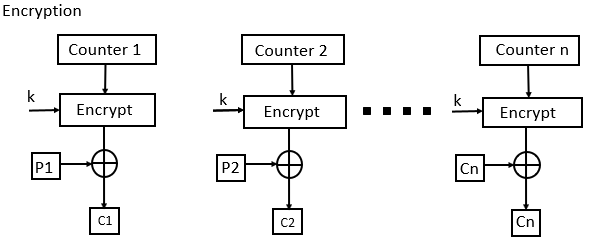
\includegraphics[width=0.5\textwidth]{KBE/img/ctr.png}
\end{figure}


\subsection{Cipher block chaining (CBC)}

Ciphertext se xoruje s plaintextem následujícího bloku, pak se to celé šifruje. Problém je, že na konci v posledním ciphertextu bude padding. A pokud správně správu zarovnáme, tak můžeme na konci kontrolovat padding.

Vezmeme ciphertext, který chceme rozklíčovat, a zjistíme, ve kterém bloku jsou data, která nás zajímají. Pak zahodíme vše, co je za nimi. Pak budeme manipulovat s posledním bytem předposledního bloku (ciphertext předposledního bloku se xoruje s plaintextem), a zkoušet posílat takový ciphertext na server. Při dešifrování vyjdou serveru v předposledním bloku kraviny, ale to nás nezajímá. Pokud na posledním místě posledního bloku bude 0x01, je to platný padding, jinak server hodí chybu.

Pokud chybu nehodí, víme, že xor posledních bytů v ciphertextu předposledního bloku a plaintextu paddingu (tedy 0x01) nám dá plaintext posledního bloku - to je to, co jsme chtěli zjistit.

Pak upravíme poslední byte předposledního bloku tak, aby nám vycházelo po xoru 0x02, a budeme měnit předposlední byte, dokud to neprojde - to znamená, že server přijal padding (0x02, 0x02), a tím získáme další byte.


\subsection{Galois counter mode - GCM}

GCM zároveň šifruje a podepisuje, používá transformace na Galoisových tělesech. Nevýhodou je, že autenticita je potvrzena až na konci přenosu (což se nehodí, třeba když chceme streamovat video). Je to jediné schéma v TLS1.3

\begin{figure}[ht!]
\centering
\begin{minipage}{.5\textwidth}
  \centering
  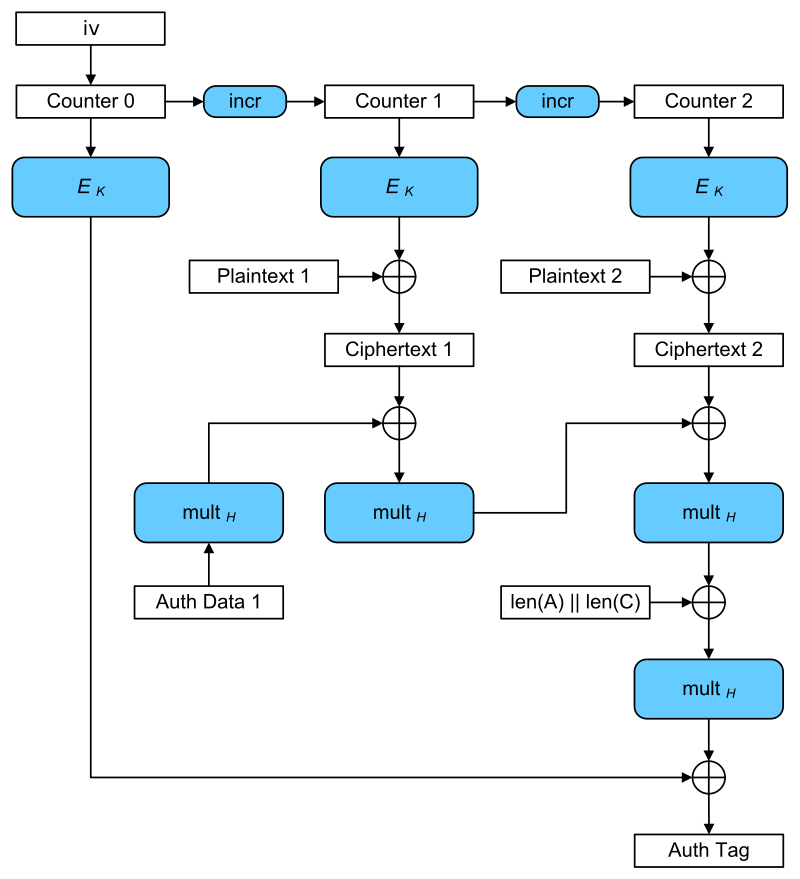
\includegraphics[width=\linewidth]{KBE/img/gcm.png}
  \caption{GCM pro blokové šifry}
  \label{fig:test1}
\end{minipage}%
\begin{minipage}{.5\textwidth}
  \centering
  \includegraphics[width=\linewidth]{KBE/img/needham-schroeder.png}
  \caption{Needham Schroederova výměna klíče}
  \label{fig:test2}
\end{minipage}
\end{figure}


\section{Needham-Schroederova výměna klíče}

DH, El Gamal, RSA a podobně jsou rozepsané v MKR, takže tady ukážu jen Needham-Shroederovu výměnu klíče, která je základem pro Kerberos. NS využívá toho, že obě strany důvěřují nějakému serveru. Každý účastník má vlastní klíč (symetrický), a jeho kopie je uložená na serveru. Alice, která chce komunikovat s Bobem, pošle serveru žádost, a server odpoví zašifrovaně (aby to nemohl přečíst nikdo jiný než Alice), a pošle v tom i klíč SK a token pro Boba. Alice pošle Bobovi token, ten je ho schopný dešifrovat svým klíčem, a pak jsou schopni komunikovat pomocí klíče SK.

Nevýhodou je, že tokeny posílané Bobovi platí věčně, není tam žádná kontrola času. Odcházející pracovník banky (Alice) si může vygenerovat několik set tokenů, uložit si je a Bob nemůže vědět, že Alice už v bance nepracuje. Dnes to je problém, ale v době vzniku NS protokolu byly počítače halové a bylo jich málo.





\section{Bitcoin a jiné měny}

\subsection{Vznik peněz}
Peníze se prvně objevily ve staré Číně nebo v Mezopotámii 2k př. n. l. Ohledně vzniku peněz jsou dvě teorie. První z nich říká, že některá z obchodovaných komodit se stala natolik významnou, že se stala použitelnou jako platidlo. Druhá teorie říká, že peníze vznikly společně s vypalovanými destičkami. Ty totiž mohly obsahovat ověřené (zapečetěné) sliby, směnky, dluhy, a tedy příslib platby. Přirozeně se pak příslib platby mohl přesunout někomu jinému.

Často byly penězi mince, které vydávala mincovna řízená panovníkem. Mince byly ražené, aby zajistily integritu. I přesto se ale s mincemi manipulovalo - lidé je ořezávali a ze získaného kovu odlévali nové mince. Mincovny v době krize šidily odlévaný kov a přidávaly do něj levnější příměsi.

\subsection{Inflace}
Moderní peníze vydávané centrálními bankami podléhají inflaci, tedy znehodnocení. To je dané tím, že objem peněz v oběhu se stále zvětšuje, jednak tiskem nových peněz, jednak půjčkami jiným bankám. Za stejný objem peněz se tedy s postupujícím časem dá koupit méně a méně zboží.

U kryptoměn se inflace nevyskytuje, protože jsou navrženy tak, aby nešly vydávat další peníze.

\subsection{Kryptoměny jako směnky}

Kryptoměny jsou založené na shodě komunity spíš než na centrální autoritě. Vypadají podobně jako směnky ze středověké Francie: \textit{Já, X, slibuji zaplatit částku Y panu Z.}

Při obchodování mohl pan Z zaplatit směnkou panu W, pokud pan W věřil tomu, že X peníze splatí. Na směnku se pak připisovali noví vlastníci. Po zaplacení byla směnka zničena. \textit{Já, Z, si přeji, aby peníze byly vyplaceny panu W.}

Obdobně v kryptoměnách vzniká blockchain, což je vlastně sekvence plateb a závazků. Kryptoměny jsou směnky, lze je dělit a dávat někomu jinému (platit).

\subsection{Eliptické křivky pro podpisy}

Pro výpočet podpisu je dán veřejný klíč $a, b, p, G, N$, kde $a, b$ jsou parametry křivky, ze které vznikla grupa, $p$ je modul, $G$ je generátor a $N$ je počet prvků v grupě (bodů na křivce).

Zvolíme náhodný soukromý klíč $d_a$ (v bitcoinu má 256bitů), a spočítáme veřejný klíč $Q_a$ jako opakované přičítání generátoru: $Q_a = d_a * G$. To je podobné jako v DSA, kde se počítalo $g^{d_a}$. Všechno počítání probíhá v modulu $p$.

Pak pro podepsání zprávy z hashem $m$ vygenerujeme nonce $k$. Spočítáme $P = k * G$, a přečteme $R$ jako x-ovou souřadnici bodu $P$. Pak podpis je $s$: $s = (m + d_a * R) * k^{-1}$.

Adresátovi se pak posílá zpráva s příslušným hashem, veřejné parametry $(a, b, p, G, N)$, klíč $Q_a$.
TODO

Při verifikaci se spočítá $P = s^{-1} * m * G + s^{-1} * R * Q_a$.

\paragraph{Důkaz správnosti}
$
P = s^{-1} m G + s^{-1} R Q_a
P = s^{-1} m G + s^{-1} R d_a G
P = s^{-1} G m + s^{-1} G R d_a
P = s^{-1} G (m + R d_a)
k = s^{-1} (m + R d_a)$

\subsection{EC a Bitcoin}

hash $Q_a$ je adresa peněženky
transakce má na vstupu předchozí transakce
na výstupu jsou transakce a poplatek

Blockchain se skládá z bloků, blok je sbírka transakcí (merkelovy stromy). Každý blok obsahuje hash předchozího bloku, tím jsou seřazeny jasně za sebe.

Další článek do bloku přidávají mineři, kteří sbírají transakce do bloku a pak se snaží najít hodnotu, která s hashem poslendího uzavřeného bloku vyjde "nějak hezky". Ten miner, kterému se to podaří nejrychleji, přidá za blockchain nový blok, a ostatní mineři nově začnou počítat s tímto blokem. Ten, kdo blok uzavře, dostane odměnu z poplatků transakcí.



\end{document}